% THIS IS SIGPROC-SP.TEX - VERSION 3.1
% WORKS WITH V3.2SP OF ACM_PROC_ARTICLE-SP.CLS
% APRIL 2009
%
% It is an example file showing how to use the 'acm_proc_article-sp.cls' V3.2SP
% LaTeX2e document class file for Conference Proceedings submissions.
% ----------------------------------------------------------------------------------------------------------------
% This .tex file (and associated .cls V3.2SP) *DOES NOT* produce:
%       1) The Permission Statement
%       2) The Conference (location) Info information
%       3) The Copyright Line with ACM data
%       4) Page numbering
% ---------------------------------------------------------------------------------------------------------------
% It is an example which *does* use the .bib file (from which the .bbl file
% is produced).
% REMEMBER HOWEVER: After having produced the .bbl file,
% and prior to final submission,
% you need to 'insert'  your .bbl file into your source .tex file so as to provide
% ONE 'self-contained' source file.
%
% Questions regarding SIGS should be sent to
% Adrienne Griscti ---> griscti@acm.org
%
% Questions/suggestions regarding the guidelines, .tex and .cls files, etc. to
% Gerald Murray ---> murray@hq.acm.org
%
% For tracking purposes - this is V3.1SP - APRIL 2009

\documentclass{sig-alternate}
%\documentclass{acm_proc_article-sp}
\usepackage{hyperref}
\usepackage[utf8]{inputenc}
\usepackage{placeins}
\usepackage{listings}
\usepackage{float}

\lstset{basicstyle=\ttfamily\tiny,breaklines=true}
\lstset{frame=single,framerule=0.1pt}

\begin{document}

\title{Enabling reactive cities with the iFLUX middleware}
%\subtitle{[Extended Abstract]
%\titlenote{A full version of this paper is available as
%\textit{Author's Guide to Preparing ACM SIG Proceedings Using
%\LaTeX$2_\epsilon$\ and BibTeX} at
%\texttt{www.acm.org/eaddress.htm}}}

%
% You need the command \numberofauthors to handle the 'placement
% and alignment' of the authors beneath the title.
%
% For aesthetic reasons, we recommend 'three authors at a time'
% i.e. three 'name/affiliation blocks' be placed beneath the title.
%
% NOTE: You are NOT restricted in how many 'rows' of
% "name/affiliations" may appear. We just ask that you restrict
% the number of 'columns' to three.
%
% Because of the available 'opening page real-estate'
% we ask you to refrain from putting more than six authors
% (two rows with three columns) beneath the article title.
% More than six makes the first-page appear very cluttered indeed.
%
% Use the \alignauthor commands to handle the names
% and affiliations for an 'aesthetic maximum' of six authors.
% Add names, affiliations, addresses for
% the seventh etc. author(s) as the argument for the
% \additionalauthors command.
% These 'additional authors' will be output/set for you
% without further effort on your part as the last section in
% the body of your article BEFORE References or any Appendices.

\numberofauthors{4} %  in this sample file, there are a *total*
% of EIGHT authors. SIX appear on the 'first-page' (for formatting
% reasons) and the remaining two appear in the \additionalauthors section.
%
\author{
% You can go ahead and credit any number of authors here,
% e.g. one 'row of three' or two rows (consisting of one row of three
% and a second row of one, two or three).
%
% The command \alignauthor (no curly braces needed) should
% precede each author name, affiliation/snail-mail address and
% e-mail address. Additionally, tag each line of
% affiliation/address with \affaddr, and tag the
% e-mail address with \email.
%
% 1st. author
\alignauthor
Olivier Liechti\\
       %\affaddr{HES-SO UAS-WS}\\
       \affaddr{HES-SO University of Applied Sciences Western Switzerland}\\
       %\affaddr{Rue de Galilée 15}\\
       \affaddr{CH - 1401 Yverdon-les-Bains}\\
       \affaddr{olivier.liechti@heig-vd.ch}
% 2nd. author
\alignauthor
Laurent Prévost\\
       \affaddr{HES-SO UAS-WS}\\
       %\affaddr{Rue de Galilée 15}\\
       \affaddr{CH - 1401 Yverdon-les-Bains}\\
       \affaddr{laurent.prevost@heig-vd.ch}
%\alignauthor Valentin Delaye\\
%       \affaddr{Novaccess SA}\\
%       %\affaddr{Rue de Galilée}\\
%       \affaddr{CH - 1401 Yverdon-les-Bains}\\
%       \affaddr{valentin.delaye@novaccess.ch}
\and  % use '\and' if you need 'another row' of author names
% 4th. author
\alignauthor Jean Hennebert\\
       \affaddr{HES-SO UAS-WS}\\
       %\affaddr{Bd. de Pérolles 80}\\
       \affaddr{CH - 1705 Fribourg}\\
       \affaddr{jean.hennebert@hefr.ch}
% 5th. author
\alignauthor Vincent Grivel\\
       \affaddr{HES-SO UAS-WS}\\
       %\affaddr{Bd. de Pérolles 80}\\
       \affaddr{CH - 1705 Fribourg}\\
       \affaddr{vincent.grivel@hefr.ch}
%% 6th. author
%\alignauthor Jean-Philippe Rey\\
%       \affaddr{HES-SO UAS-WS}\\
%       %\affaddr{CH - Rue de Galilée 15}\\
%       \affaddr{1401 Yverdon-les-Bains}\\
%       \affaddr{jean-philippe.rey@heig-vd.ch}
%\and
%\alignauthor Jonathan Depraz\\
%       \affaddr{Novaccess SA}\\
%       %\affaddr{Rue de Galilée}\\
%       \affaddr{CH - 1401 Yverdon-les-Bains}\\
%       \affaddr{jonathan.depraz@novaccess.ch}
%\alignauthor Marc Sommer\\
%       \affaddr{Novaccess SA}\\
%       %\affaddr{Rue de Galilée}\\
%       \affaddr{CH - 1401 Yverdon-les-Bains}\\
%       \affaddr{marc.sommer@novaccess.ch}
}


% There's nothing stopping you putting the seventh, eighth, etc.
% author on the opening page (as the 'third row') but we ask,
% for aesthetic reasons that you place these 'additional authors'
% in the \additional authors block, viz.
%\additionalauthors{Additional authors: John Smith (The Th{\o}rv{\"a}ld Group,
%email: {\texttt{jsmith@affiliation.org}}) and Julius P.~Kumquat
%(The Kumquat Consortium, email: {\texttt{jpkumquat@consortium.net}}).}
%\date{30 July 1999}
% Just remember to make sure that the TOTAL number of authors
% is the number that will appear on the first page PLUS the
% number that will appear in the \additionalauthors section.

\maketitle
\begin{abstract}
This paper presents the iFLUX middleware, designed to provide a lightweight integration solution for Smart City applications. Based on three core abstractions, namely \emph{event sources}, \emph{action targets} and \emph{rules}, iFLUX makes it very easy to expose sensors and actuators through REST APIs so that they can be integrated in application-level workflows. Sensors and actuators can be smart objects integrating hardware and software, but can also be pure software services. In the paper, we introduce the iFLUX programming model and describe how it has been implemented in a middleware platform. We also report on how the platform has been used and evaluated in various contexts. While iFLUX has been initially designed in the context of Smart City applications, it is generic and applicable to other domains where hardware and software components are connected through the Web.

\end{abstract}

\keywords{smart city, integration middleware, rule engine}

\section{Introduction}

While there is no single definition for the term \emph{Smart City} \cite{caragliu2011smart,batty2012smart,shapiro2006smart}, the general idea is that ICT technologies can contribute to improve the quality of life by impacting a wide range of domains: energy, transport, safety, administration, politics, culture, etc. Because of this broad definition, very different types of applications and technologies fit in the scope of smart cities. Think of a sensor network that measures air quality. Think of an application that optimizes public transportation usage by giving incentives to travel outside peak hours. Think of services that encourage citizen to interact more actively and directly with authorities. These are only a few examples that illustrate the variety of smart city applications. Some of these applications have a strong physical dimension, when sensors and actuators are material artifacts (smart objects). Other applications have a lesser physical dimension, when the sensors and the actuators are actually software systems (e.g. mobile applications, online business services). In this paper, we consider the entire spectrum between these two cases.

Cities do not become \emph{smart} overnight. Rather, they become smarter through an evolutionary process. New technologies and applications are introduced over a long period of time, often without an overall architecture defined a priori. Every domain of the city is managed as a silo, with its own needs, its own services and its own infrastructure. For this reason, it is often difficult to build cross-domain applications. Think of an application that would seek to optimize energy consumption by continuously adapting street lighting to the current road traffic. While the sensors (on the roads) and the actuators (in the street lights) might actually be deployed, building the application is generally a challenge because the two components live in two silos, isolated because of a mix of organizational, administrative and technical reasons.

This situation is analogous to any significant information system. Hence, it raises the usual questions: what is the best way to integrate heterogenous components deployed across a Smart City? How can we enable developers to create and deploy new services independently, while ensuring that these services can be shared, reused and combined in higher-level workflows and applications? How can we make the integration of legacy services into the new ecosystem as effortless as possible? Over the last decade, the REST architectural style and standard web technologies (HTTP, JSON, etc.) have proven to be very effective in this pursuit. Combined with the exponential growth of the Internet of Things both in consumer and industrial settings, this makes the Web of Things \cite{Guinard2009} an ideal paradigm for designing city-wide services, where there is a mix of hardware and software components.

Adopting the Web of Things as an architectural style for smart city applications, however, does not address all architectural questions. What concrete guidelines should be followed to expose components through REST APIs? What interaction patterns should be used between system components? How can we concretely ease the creation of new urban services? How do we ensure that the interaction with these services in higher-level applications is easy and manageable? It is to investigate such issues that the iFLUX project has been initiated. Our first objective was to propose a programming model, based on WoT principles, that can be applied to build citywide applications. Our second objective was to expose this programming model in a concrete middleware platform and to evaluate it in a series of illustrative applications.

In the remaining sections of this article, we first give more information about the context in which iFLUX has been created and describe the main design objectives associated with this context. We then introduce the iFLUX programming model by describing three core concepts: \emph{event sources}, \emph{action targets} and \emph{rules}. We then present one aspect of the middleware implementation, by describing three main RESTful endpoints. We finally explain how we have evaluated the platform in several applications, some of which have been built by third-party developers.

\subsection{iFLUX on GitHub}

All the work done in the iFLUX project is in Open Source on GitHub. The main repository, which has references to all others, is \url{https://github.com/SoftEng-HEIGVD/iflux-docker}. You will find all the close to far related projects from this one. Read the different readme present in each repository to get specific details.
\section{Context and design objectives}

The need for the iFLUX middleware has emerged in a research program dedicated to smart cities, entitled iNUIT and established at the HES-SO University of Applied Sciences Western Switzerland. The goal of iNUIT is to build a complete IoT stack for smart city applications. It is based on a layered architecture: the lower layer deal with the interconnection of physical objects (specialized sensors, low-power mesh networks, WoT gateways, etc.), the intermediate layer deal with data analysis (sensor fusion, video processing, etc.) and the upper layer hosts applications (e.g. crowd monitoring). Initially, middleware services have been provided in the iNUIT cloud for archiving and querying information (both raw sensor data and extracted information). One goal of iFLUX was to add the capability to process event streams and to enable a reactive programming style \cite{reactive}.

\subsection{Reuse}

Our first objective was to encourage the reuse of iNUIT services developed in different projects. Typically, the teams working on individual components (e.g. a new type of sensor, a video processing module) focus on a specific service. They often implement basic demonstrators to validate this service. What is often not so easy to do for them is to expose the service, so that it can be found and used by other teams (and in particular by those working at the application level). Hence, our first goal was to provide an easy solution for component developers to bring their technology in a single service catalog. From the application developers point of view, the interaction with all services in the catalog should follow the same approach and patterns. This is what is captured in the iFLUX programming model.

\subsection{Decoupling}

The fact that many independant teams are involved in the iNUIT program reflects what happens in most smart city environments, from an organizational point of view. In the introduction, we used the term \emph{silo}, to suggest that it must be possible for different teams to develop atomic services and applications with as few dependencies as possible. With this in mind, iFLUX is based on a micro-services oriented architecture. Every component of the ecosystem is developed and operated independently. Web protocols provide the platform-independant glue between the components. We have used the Docker virtualization technology, based on lightweight containers, to facilitate the packaging and deployment of these independent components.

\subsection{Simplicity}

We wanted iFLUX to be very lightweight and easy to use, both for service and application developers. The programming model should be easy to grasp, hence with a small number of abstractions. Bringing a sensor or an actuator into the iFLUX ecosystem should not require a big effort. The APIs that have to be consumed or published should be concise. This is one reason for which we have decided to initially only support stateless rules. We will later show that state can easily be managed in \emph{action targets}.
\section{Programming model}

The programming model for iFLUX was inspired from popular lightweight service integration services, such as IFTTT \cite{ifttt}  and Zapier \cite{zapier}. It follows the Event Condition Action (ECA) paradigm \cite{bailey2004event,qiao2007developing,papamarkos2003event} and is based on three core abstractions: i) \emph{event sources}, ii) \emph{action targets} and iii) \emph{rules}. \emph{Event sources} and \emph{action targets} are meant be developed by third-party developers, independently from any specific application (to encourage reuse). Application developers implement workflows on top of available \emph{event sources} and \emph{action targets}, by defining stateless rules. Essentially, they express rules such as ``\emph{if} an event with properties that match these conditions is notified, \emph{then} trigger an action on this target, with the following properties".

In addition, we have extended the concept of \emph{Event Sources} and \emph{action targets} by a template mechanism. The idea behind this template mechanism is, for instance, to let the user defining an event source template which will be instantiated to an real event source. In this context, the template is the definition of the event source or the action target. An instance of an event source or an action target is the real system sending the events or receiving the actions. In addition, the instance let the possibility to customize the configuration through a callback defined on the event source or the action target. This will be covered later.

\subsection{Event Source Templates}
\label{sec:est}

An \emph{event source template} is a type of autonomous component that produces a stream of typed events. Based on this definition, there are quite different types of event source templates. Here are some examples:

\begin{itemize}
\item \emph{Connected hardware sensors} that emit a continuous flow of low-level events. In this case, the events are observations or measures captured by the sensors.
\item \emph{Software sensors} that capture some kind of activity in a digital system and emit related events. For instance, one can think of a software sensor embedded in a business application that emits an event whenever a business-level condition is met.
\item \emph{Data processing services} that emit higher-level events. Typically, a data processing service aggregates several streams of low level events and applies some kind of logic to produce a new stream.
\item \emph{User agents} used as proxy to emit human generated events. For instance, think of a mobile application used to report incidents.
\end{itemize}

\subsection{Event Sources}
\label{sec:es}

An \emph{event source} is an instance of an \emph{event source template}. This will represent a unique and specific source of typed events. Based on this definition, there are quite different types of event sources. 

All the previous examples are valid in the way that each sensor is uniquely identified and represent a stream of events. Therefore, you can have several temperature sensor which represent the save event source template so the same kind of events will be triggered but each event comes from a specific sensor. In the case of the data processing service, it will allow scoping the events stream to a data context.

The iFLUX middleware exposes a standard REST API that \emph{event sources} use to stream their data. The API specifies a simple payload structure: an event is defined by a timestamp, a source, a type and a list of properties. The list of properties depends on the event type.

\subsection{Action Target Templates}
\label{sec:att}

An \emph{action target template} is a component that exposes logic that can be triggered from the iFLUX middleware. Here also, there are different types of action target templates:

\begin{itemize}
\item \emph{Connected hardware actuators} that can be remotely controlled. A smart street light or a large public display located in a stadium are two examples.
\item \emph{Software actuators} that are typically business applications or gateways deployed for integration purposes.
\item \emph{User interaction channel gateways} that are special software actuators geared at delivering notifications to people. Examples include gateways for delivering e-mails, push notifications and social network notifications.
\end{itemize}

\subsection{Action Targets}
\label{sec:at}

An \emph{action target} is an instance of an \emph{action target template}. This time, this will allow to create action streams dedicated to an instance of action target.

For example, you can have a light actuator action target template which is instantiated in each room of a building. With the proper rule and the proper light sensor, we will be able to switch on or off the light in the correct room.

The developers of \emph{action targets} must implement a simple REST API and process incoming action payloads. An action payload is defined by a timestamp, a type and a list of properties.

\subsection{Rules}
\label{sec:rules}

The last abstraction in the iFLUX model is the notion of rule. Rules are what bind events and actions together. A rule specifies that \emph{if} an event is notified and its properties meet certain criteria \emph{then} one or more actions has to be triggered with a list of properties (which values are computed based on the event properties).
\section{Implementation}

Since the first version of iFLUX, where we apply the \emph{lean} and \emph{agile} principles, we continued to apply these methodologies. Therefore, for the second version of iFLUX, we delivered feature after feature as fast as possible. We wanted to have something that we and others could experiment with rapidly, so that we would rapidly benefit from feedback. After few months, we have been able to implement a whole system with various demonstrators. We were able to assemble the different pieces by specifying rules. 

The very first user interface only provided a mechanism to create \emph{rules} and to simulate their evaluation. We have the possibility to enable the configuration of \emph{event sources} and \emph{action targets} as well. We now do most of our development on top of the Node.js platform, but we also SDKs in other languages.

\subsection{Architecture}

Since the project inception, we have relied on virtualization technologies, such as Vagrant and Docker, to make it easy for third-party developers to have a working environment on their machines. We introduced few technologies to let iFLUX be scalable. We introduced Kafka for the messaging bus letting the events be handled totally asynchronously. We received the events on a gateway dedicated to that and consume them on iFLUX rule engine. Therefore, a high charge of events will not be an issue as the cost to accept them is really small. We have also setup ElasticSearch to gain the possibility to use his full text capabilities. It is also an additional debug tool to see when and where the events comes and goes. You can refer to Figure \ref{fig:iflux-archi} to see the overall core architecture of the system.

\begin{figure}
\centering
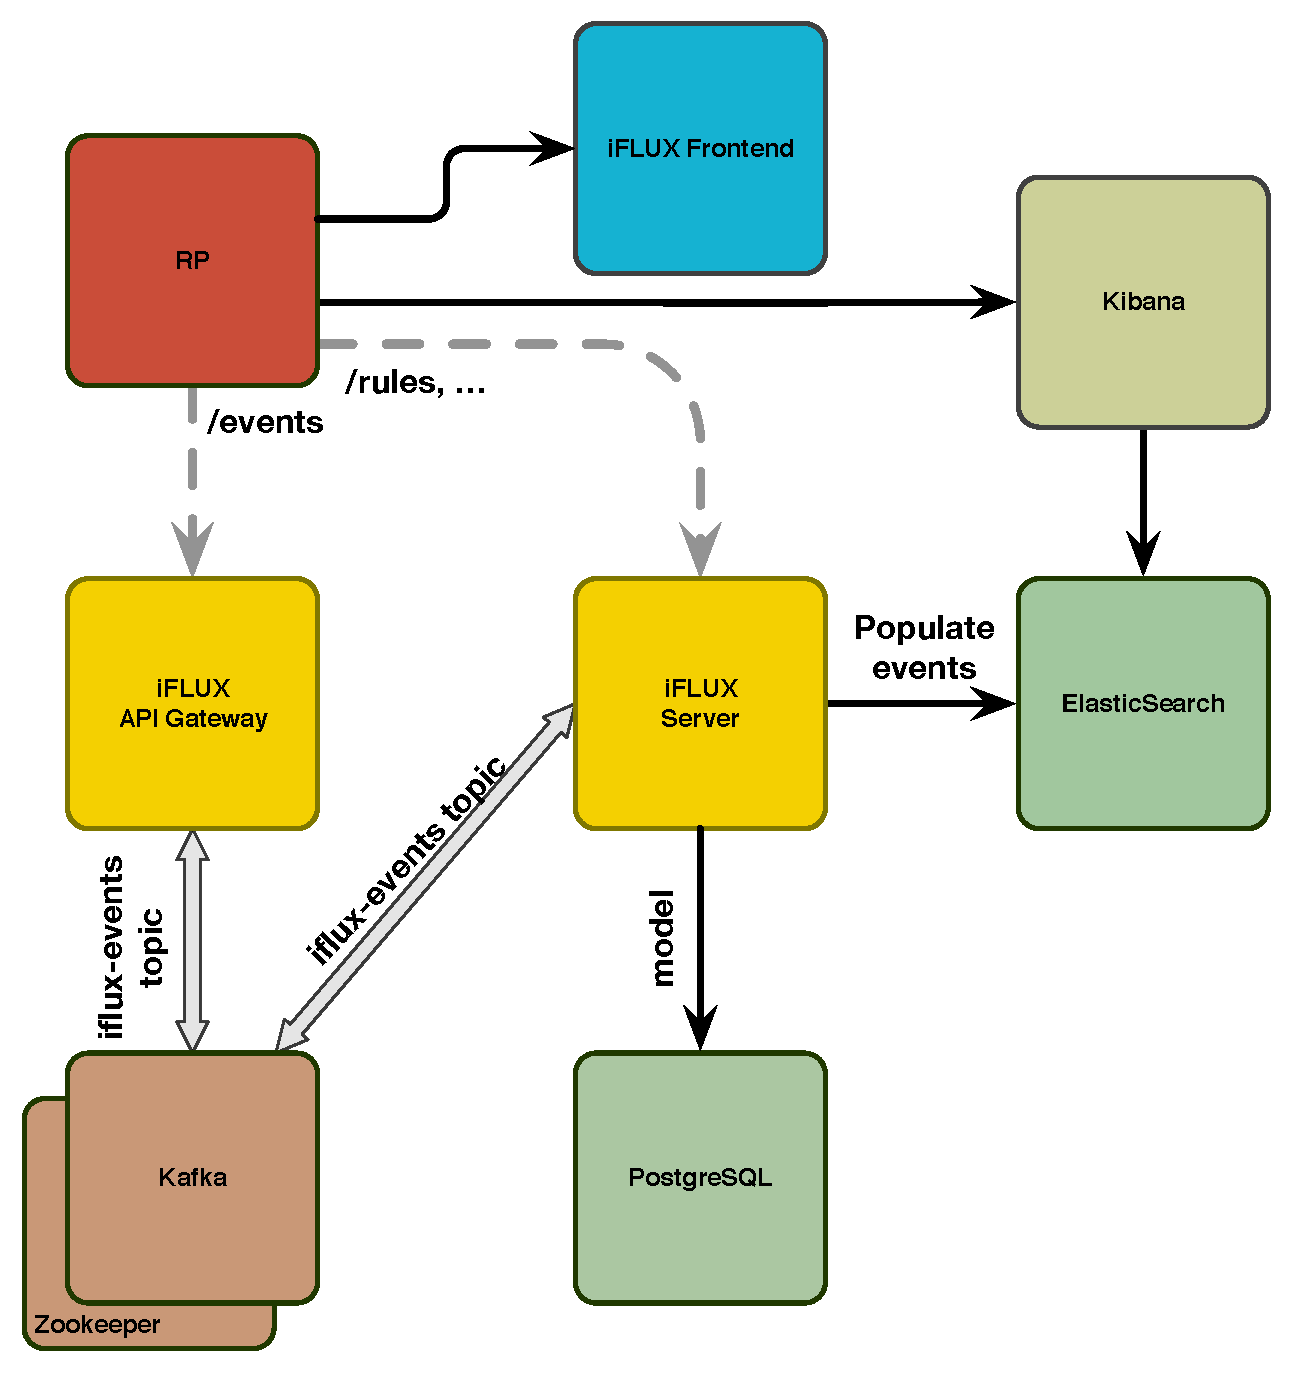
\includegraphics[width=1\columnwidth]{figures/iflux-archi.pdf}
\caption{The iFLUX architecture}
\label{fig:iflux-archi}
\end{figure}

\subsubsection{Reverse Proxy}

The reverse proxy receive all the inbound traffic and direct the requests to the right components. Kibana, iFLUX Frontend, iFLUX Gateway and iFLUX Server are accessible through the reverse proxy.

\subsubsection{iFLUX Frontend}

The frontend is the visual configuration tool of iFLUX. It offers CRUD operations through an Angular application to manipulate the iFLUX model. You can define event sources, action targets, rules and all required models.

\subsubsection{iFLUX API Gateway}

This gateway, today, offers only the \emph{/events/} API to accept quickly the events from the outside world without blocking any external system. This server is stateless and have no data store. The events received are forwarded to iFLUX Server through the message bus offered by Kafka.

\subsubsection{Kafka and Zookeeper}

We use Kafka to have a message bus to let the events to be handle asynchronously by the rule engine on the iFLUX Server. This component in the architecture let iFLUX to scale.

\subsubsection{iFLUX Server}

iFLUX Server manage the data models and has the rule engine. The rules are evaluated each time an event is received through the message bus. Once a rule is evaluated positively, action are triggered. But before an evaluation is done, the event received is stored in ElasticSearch for later analysis purpose. The result of the evaluation is also stored in ElasticSearch in a second index. The data model is stored in a PostgresSQL database.

\subsubsection{PostgresSQL}

Data backend of iFLUX. All the action targets, event sources, rules and so on are stored in this database. We do not store in this relational database any of the received events.

\subsubsection{ElasticSearch}

We use ElasticSearch to store the events and the result of the rules evaluation to make text searches and data analysis in the time. 

\subsubsection{Kibana}

Finally, Kibana is the frontend of ElasticSearch letting us to make text searches, to view graphs and trends on the events received and the evaluation results.

\subsection{REST APIs}

In addition of the three core abstraction of the iFLUX programming model, there are several additional resources exposed through the REST API. The endpoints are described in the following list: 

\begin{itemize}
\item \textbf{/auth} the authentication endpoint allow the users to register or sign in;
\item \textbf{/health} just an API to let the user to get the version of iFLUX core and to know the server is working;
\item \textbf{/actionTargets} where to manage the action targets;
\item \textbf{/actionTargetTemplates} where to manage the template of the action targets;
\item \textbf{/eventSources} where to manage the event sources;
\item \textbf{/eventSourceTemplates} where to manage the template of the event sources;
\item \textbf{/eventTypes} where to manage the event types;
\item \textbf{/me} where to get some info about himself;
\item \textbf{/organizations} where organization are managed. All in the iFLUX core is scoped to the organizations;
\item \textbf{/rules} where to manage the rules;
\item \textbf{/schemas} where to retrieve the JSON Schema used by the different iFLUX models;
\item \textbf{/events} not part of the iFLUX core directly as it is implemented on the gateway. But it is part of the general iFLUX API.
\end{itemize}

Apart from those endpoints, the event sources and the action targets, when required, must offer an API to configure the instances. On the action targets, an API to accept triggered action must be implemented.

\subsubsection{The \texttt{/events/} endpoint}

This endpoint and the payload that it accepts is straightforward. Every iFLUX \emph{event source} produces a stream of events. It POSTs these events on the endpoint. Notice that the payload accepts an array of events, so it is possible to send several events in a single request. For every event, there is a timestamp, a source (an ID to an event source), a type (a link to a JSON schema) and an array of custom properties. As you can see, writing an iFLUX event source is very simple. In particular, bringing an existing component (WoT gateway, mobile app, business application, etc.) into the iFLUX ecosystem is not a burden, which was one of our main design objectives. Furthermore, this can be done on any kind of platform (software and firmware), since the only requirement is to be able to issue an HTTP request.

\begin{lstlisting}
POST /events/ HTTP/1.1
Content-type: application/json

[
  {
    "timestamp" : "2015-01-12T05:21:07Z",
    "source" : "JI8928JFK",
    "type" : "http://localhost/eventTypes/temperatureEventSchema",
    "properties" : {
      "temperature" : 22.5,
      "location" : "room 1"
    }
  },
  {
    "timestamp" : "2015-01-12T05:22:07Z",
    "source" : "JI8928JFK",
    "type" : "http://localhost/eventTypes/temperatureEventSchema",
    "properties" : {
      "temperature" : 22.8,
      "location" : "room 1"
    }
  }
]
\end{lstlisting}

\subsubsection{The \texttt{/configure/} endpoint}

In the case of event source and action target that requires a dedicated configuration, iFLUX core will call the \texttt{/configure/} on the remote host. This remote endpoint should offer the API.

The action target must let the possibility to set an action target ID and a bunch of free properties.

\begin{lstlisting}
POST /configure/ HTTP/1.1
Content-type: application/json

{
  "target" : "8JFKJI892",
  "properties" : {
    "periodicity" : "daily"
  }
}
\end{lstlisting}

The event source must let the possibility to set an event source ID and a bunch of free properties.

\begin{lstlisting}
POST /configure/ HTTP/1.1
Content-type: application/json

{
  "source" : "JI8928JFK",
  "properties" : {
    "sensorId" : "thermo-1"
  }
}
\end{lstlisting}

\subsubsection{The \texttt{/actions/} endpoint}

This endpoint is analogous to the events endpoint. It has to be implemented by every \emph{action target}, to expose functionality that can be triggered when iFLUX rules are evaluated positively. Here again, it is possible to send several action payloads in a single HTTP request. Every action has a type (a link to a JSON schema) and a list of custom properties that depend on this type. Notice that there is no link to the action target, since this information is already part of the action resource URL (e.g. \url{https://myactuator.mysystem.com/actions/}). It must also contains the action target ID to identify which instance will be triggered. In case the action target is not configurable, the action target ID is sent anyway but should be skipped.

\begin{lstlisting}
POST /actions/ HTTP/1.1
Content-type: application/json

[
  {
    "target": "8JFKJI892",
    "type" : "http://localhost/actionTypes/sendAlertViaEmailSchema",
    "properties" : {
      "email" : "user.name@iflux.io",
      "subject" : "Alert: something has happened!",
      "body" : "An event has been notified to iFLUX by a source and a rule states that we should inform you about it."
    }
  },
  {
    "target": "8JFKJI892",
    "type" : "http://localhost/actionTypes/sendAlertViaEmailSchema",
    "properties" : {
      "email" : "user.name@iflux.io",
      "subject" : "Alert: something has happened!",
      "body" : "An event has been notified to iFLUX by a source and a rule states that we should inform you about it."
    }
  }
]
\end{lstlisting}

\subsubsection{The \texttt{/rules/} endpoint}

This endpoint is used to perform CRUD operations of iFLUX rules. Unlike the previous endpoints, which only accept POST requests, it accepts GET, POST, PATCH and DELETE requests. In addition to the simple metadata (a description and a reference), every rule has two parts: the \emph{conditions} part and the \emph{transformations} part. The \emph{conditions} part specifies under which conditions the rule will be fired. It is possible (but not mandatory) to specify an event source, an event type and a list of property values. In other words, it is possible to define rules that are fired ``\emph{if any sensor sends an event with a temperature above 30 degrees}" or ``\emph{if the particular sensor in my kitchen sends any kind of event}". The \emph{transformations} part specifies which action(s) should be triggered on which \emph{action target(s)} when the rule is fired. The property \texttt{actionSchema} contains a javascript expression, which specifies how to create the action payload based on the event properties.

\begin{lstlisting}
POST /actions/ HTTP/1.1
Content-type: application/json

{
  "description" : "When a temperature event is received, notify Bob by email.",
  "reference": "TEMPERATURE-EMAIL-NOTIFICATION",
  "enabled": true,
  "conditions" : [{
    "eventSourceId" : 12,
    "eventTypeId" : 1
  }]
  "transformations" : [{
    "actionTargetId" : 28,
    "fn": {
    	"expression": "return { "temp": event.properties.temperature };"
    }
  }]
}\end{lstlisting}

\subsubsection{The other endpoints}

The GitHub repositories of iFLUX contains the API documentation which is more complete than the description given in this document. You should take a look on \url{https://github.com/SoftEng-HEIGVD/iflux-apidoc} or \url{https://iflux.heig-vd.ch/doc/} to have a deeper view on the APIs. You will realize that most of the APIs are CRUD oriented.

\subsection{The data model}

In iFLUX, we manipulate various data stored in a PostgreSQL database. The data stored are only related to the rules. No event is stored directly in iFLUX. In place, for the events, we rely on on ElasticSearch.

The Figure \ref{fig:data-model} presents the different models. In fact, this is really similar to the APIs. We have the organizations to scope all the data visibility to only members of the organizations. Action target and their templates like the event sources and their templates can be public or not. When they are defined as public, they become usable by every iFLUX registered users. Changing the visibility of any of this model will only prevent them to be used in the future. In figure, the dashed lines will refer to weak links meaning that the link is defined only in the code and not through database integrity constraints.

\begin{figure}
\centering
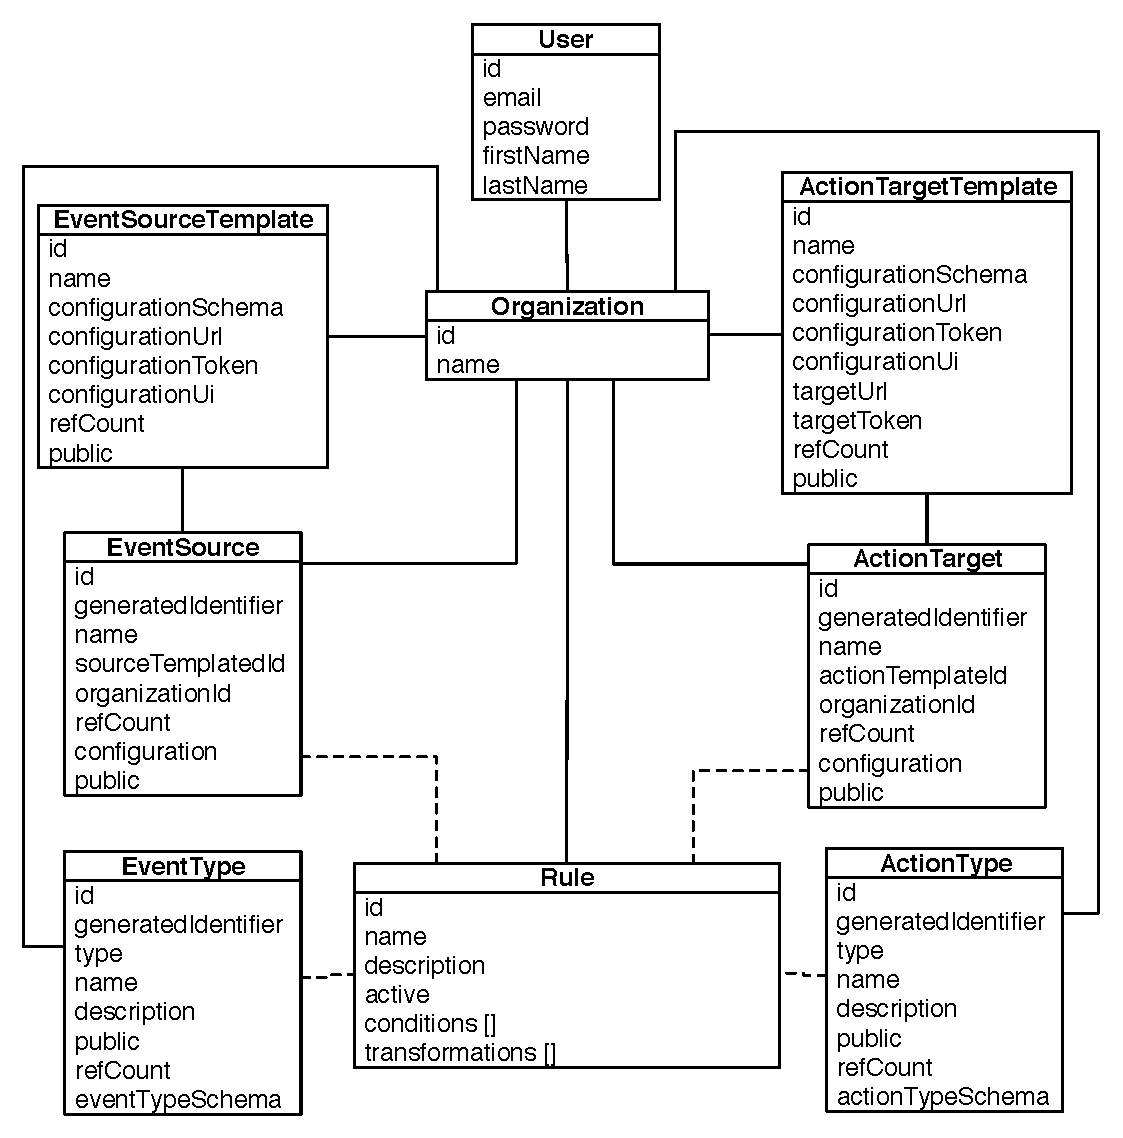
\includegraphics[width=1\columnwidth]{figures/data-model.pdf}
\caption{The iFLUX data model}
\label{fig:data-model}
\end{figure}

\subsubsection{Commons attributes}

In the next few sections, we will describe the different models of iFLUX. Some of them share the same attributes dedicated to the same usage. Therefore, we will describe them below:

\begin{itemize}
\item \textbf{generatedIdentifier} This a unique string across a model generated on the server side which is not editable by iFLUX users;
\item \textbf{refCount} this field is a cache of the number of times the model is referenced by another model. This is a shortcut to let the UI knowing if the model can be deleted or not;
\item \textbf{*Schema} in general, all the attributes terminated by the suffix Schema refers to a JSON Schema;
\item \textbf{*Token} when we talk about tokens in our models, this means that we expect a token that will be used in the HTTP header \emph{authentication} with a sort of \emph{bearer}; It is not yet possible to specify other security authentication schemes;
\item \textbf{public} when public flag is present, it means that the model can be kept private when set to false and therefore the model remains visible only by members of the same organization. If set to true, the model is visible by everybody in iFLUX. Only members of an organization can edit/delete models owned by the organization even if they are public.
\end{itemize}

\subsubsection{Organizations}

The organization is the main model in iFLUX. All the remaining data are scoped to the organizations. There is no way to transfer a model from an organization to another organization. In place of that, we have a public/private mechanism which allows to open the usage (not the edition) to everyone.

An organization is defined by a name that must be unique across the system.

\subsubsection{Users}

Users are automatically a member of at least one organization. There is no concept of privileges in an organization. Being part of an organization will allow the member to do everything in the organization. This means that any member can create, read, update or delete any model attached to the organization where the user is a member.

A user is defined by a first name, a last name and an email. In addition, the user has to set a password that will be stored ciphered in the database.

\subsubsection{Event Source Templates}

The event source templates define an event source that can be instantiated multiple times in the system. Refers to \ref{sec:est} for more details.

An event source template is composed of a name that is unique in the organization, a configuration schema. This schema define the JSON payload that the external system expect when the configuration callback is used. An optional configuration token can be set. In addition, a configuration UI schema is defined optionally to offer the possibility of the frontend to prepare a corresponding UI to make the configuration. Finally, they are ref count and public attributes.

\subsubsection{Event Sources}

Event sources are instances of event source templates. This will allow to define multiple event sources on the same model. For instance, you define an event source template to be a thermometer which can send temperature events. Then, you can define one or more real thermometers uniquely identified. Fore more details, check the section \ref{sec:es}.

An event source have a name that is unique across the event sources scoped to the organization. A reference to the event source template and an organization. The configuration is the real values that will be used to configure the instance of the event source template in the remote system. Finally, the attributes generated identifier, public and ref count are present.

\subsubsection{Event Types}

The event types define the structure of the events that an event source will produce. They are used to specify the data send from an event source and then letting the definition of rules to know which data available in the action.

An event type has a name that is unique across the organization and human description is possible. The event type schema is the format of events from that type. The type is the URL to refer the schema. If the URL refer to an external service, the schema can be blank. The attributes public, ref count and generated identifier are present.

\subsubsection{Action Target Templates}

The action target templates define an action target that can be instantiated multiple times in the system. Refers to \ref{sec:att} for more details.

An action target template is composed of a name that is unique in the organization, a configuration schema. This schema define the JSON payload that the external system expect when the configuration callback is used. An optional configuration token can be set. In addition, a configuration UI schema is defined optionally to offer the possibility of the frontend to prepare a corresponding UI to make the configuration. In addition, a target URL and its optional token is required for the action callbacks which is different from the configuration callback. Finally, they are ref count and public attributes.

\subsubsection{Action Targets}

Action targets are instances of action target templates. This will allow to define multiple action targets on the same model. For instance, you define an action target template to be a light which can send be switched on/off. Then, you can define one or more real lights uniquely identified. Fore more details, check the section \ref{sec:at}.

An action target have a name that is unique across the action targets scoped to the organization. A reference to the action target template and an organization. The configuration is the real values that will be used to configure the instance of the action target template in the remote system. Finally, the attributes generated identifier, public and ref count are present.

\subsubsection{Action Types}

The action types define the structure of the actions sent to action targets. It will help to define rules with the correct action data format in the JavaScript expressions.

An action type has a name that is unique across the organization and human description is possible. The action type schema is the format of actions from that type. The type is the URL to refer the schema. If the URL refer to an external service, the schema can be blank. The attributes public, ref count and generated identifier are present.

\subsubsection{Rules}

The rules do the relations between the event sources and the actions targets as it was explained section \ref{sec:rules}.

A rule is defined by a unique name across the organization and an optional human description. The active flag is used to enable/disable the evaluation of a rule.The conditions and transformations arrays are JSON arrays stored directly in the model. Therefore, there is no strong links with integrity constraints. 

The conditions is a list of \emph{if} with the following data structure. Only one condition evaluated to true is enough to match the rule.

\begin{lstlisting}
"properties": {
  "description": {
    "description": "Human friendly text to explain the condition.",
     "type": "string"
  },
  "eventSourceId": {
    "description": "Reference to event source. If blank, * is used.",
    "type": "integer"
  },
  "eventTypeId": {
    "description": "Reference to event type. If blank, * is used",
    "type": "integer"
  },
  "fn": {
    "description": "JavaScript expression. Can be blank.",
    "type": "object",
    "properties": {
      "expression": {
        "description": "MUST be a valid JavaScript expression",
        "type": "string"
      },
      "sampleEvent": {
        "description": "A valid event to be evaluated to true with the expression.",
        "type": "object"
      }
    },
    "required": [ "expression", "sample" ]
  }
}
\end{lstlisting}

and an example:

\begin{lstlisting}
"conditions": [{
  "description": "Match if a temperature has changed.",
  "eventSourceId": 1,
  "eventTypeId": 1,
  "fn": {
    "expression": "return event.temperature.old != event.temperature.new;",
    "sampleEvent": {
      "temperature": {
        "old": 12,
        "new": 13
      }
    }
  }
}]
\end{lstlisting}

The transformations is a list of \emph{then} with the following data structure. All the transformations will be applied.

\begin{lstlisting}
"properties": {
    "description": {
      "description": "Human friendly text to let the possibility to explain the transformation.",
      "type": "string"
    },
    "actionTargetId": {
      "description": "Reference to action target.",
      "type": "integer"
    },
    "actionTypeId": {
      "description": "Reference to action type.",
      "type": "integer"
    },
    "fn": {
      "description": "JavaScript expression to create the action content.",
      "type": "object",
      "properties": {
        "expression": {
          "description": "MUST be a valid javascript expression",
          "type": "string"
        },
        "sample": {
          "description": "A valid context to evaluate the transformation",
          "type": "object",
          "properties": {
            "event": {
              "description": "A valid event.",
              "type": "object"
            },
            "eventSourceTemplateId": {
              "description": "A reference to the event source template. Can be blank.",
              "type": "integer"
            },
            "eventTypeId": {
              "description": "A reference to the event type. Can be blank.",
              "type": "integer"
            }
          },
          "required": [ "event" ]
        }
      },
      "required": [ "expression", "sample" ]
    }
  },
  "required": [ "actionTargetId", "actionTypeId" ]
}
\end{lstlisting}

and an example:

\begin{lstlisting}
"transformations": [{
  "description": "Prepare a message for Slack with the old and new temperature",
  "actionTargetId": 1,
  "eventTypeId": 1,
  "actionTypeId": 1,
  "fn": {
    "expression": "return { message: 'The temp. changed from ' + event.temperature.old + ' to ' + event.temperature.new + '.' };",
    "sample": {
      "event": {
        "temperature": {
          "old": 12,
          "new": 14
        }
      },
      "eventSourceTemplateId": 1
    }
  }
}]
\end{lstlisting}

\subsection{Model summary}

In fact, the data model of iFLUX is not so complex. A lot of things that are present for the event side are also present in the action side. Only few details change between them. The logic behind this is that it is more easy to maintain and to factorize the code if the things are close. The difference between event and action sides is mainly due to the fact that the event side is an input stream in iFLUX and the action side is an output stream. Then, the action side models require more configuration than event side.




















\section{Technologies}

During the project, we used a variety of technologies to achieve different objectives. For example, we use Docker to manage the whole architecture for the development and the production environments.

\subsection{Docker}

What is Docker? \emph{Docker is an open platform for building, shipping and running distributed applications. It gives programmers, development teams and operations engineers the common toolbox they need to take advantage of the distributed and networked nature of modern applications.}

In iFlux, we prepared several images to instantiate containers on a dedicated VM. Why using Docker? In fact, there are few reasons. Firstly, we can prepare images ready to deploy for other organizations. As the image is self contained, with just few environment variables we are able to instantiate multiple instances of iFLUX easily without having to worry about the deployment itself.

In fact, the iFLUX image, everything is already ready. We have the installation of NodeJS which the runtime that runs our application. All the application dependencies are also bundled as the application is installed. The difference between a dockerized application and a traditional one is that the bundle you ship is self contained and there is nothing to worry about. No more issues with missing dependencies or dependency repository down.

Secondly, it brings a real advantage for the deployment time. As you have your application ready to use and you have just to run one line command to run your containerized application, you have just to download it and to run it. So you can repeat this process on each environment where you want to deploy the app. In our case, we have deployed two distincts production environments. In summary, we can say prepared once, deploy everywhere.

There is the Docker image file of the iFLUX main server.

\begin{lstlisting}
# Base image which contains node installed
FROM node:0.12.6-wheezy

# Install some dependencies globally to have them in the path
RUN npm install -g grunt bower knex

# Install dependencies with a caching mechanism to improve the Docker image build process
ADD package.json /tmp/package.json
RUN cd /tmp && npm install
RUN mkdir -p /nodejs/iflux && cp -a /tmp/node_modules /nodejs/iflux

# Copy the application in the image
ADD . /nodejs/iflux

# Prepare the user stuff to run the app
RUN useradd -m -r -U iflux \
	&& chown -R iflux:iflux /nodejs/iflux \
	&& chmod +x /nodejs/iflux/start.sh

# Switch the user to let have less privileges than root user
USER iflux

# Set the working directory
WORKDIR /nodejs/iflux

# Expose the application port
EXPOSE 3000

# This instruction will be used when the container will instantiated
CMD ./start.sh
\end{lstlisting}

The script that will be run once the container is instantiated is the following.

\begin{lstlisting}
#!/bin/bash

# Run the database migration. Ensure that the database is ready each time the application is updated and redeployed
knex migrate:latest

# Start the application. Remember we are in the working directory where the application is deployed.
npm start
\end{lstlisting}

\subsubsection{Docker Compose}

We did the work to create the images for each component of iFLUX. For the database, the different action targets and event sources. Pretty much everything is dockerized. Therefore, we need an orchestration tool to manage all the containers. For that, Docker is shipped with a tool called Docker Compose. This tool allow us to prepare a configuration. The configuration contains the definition of each service and their dependencies. With that, Docker Compose is able to calculate the start order regarding the dependency graph. For example, Docker Compose will start the database used by iFLUX before the server will start.

\label{lst:docker-compose-conf}
\begin{lstlisting}
# The API documentation is exposed through static website on port 4000
ifluxapidoc:
  image: softengheigvd/iflux-apidoc:latest
  env_file: ./.env
  ports:
    - "4000:4000"

# This is a container to handle the data of all the service. In real production use case, each service will have its own data container. With this configuration, the storage is stored on the host running Docker containers and then will ensure the data are persisted between to run of a container.
ifluxsrvdata:
  build: iflux-server-data
  volumes:
    - "/iflux/db/mongo:/data/db"
    - "/iflux/db/postgres:/var/lib/postgresql/data"
    - "/iflux/kafka:/kafka"
    - "/iflux/esearch:/usr/share/elasticsearch/data"
    - "/iflux/slack:/data/slack"
    - "/iflux/viewbox:/data/viewbox"
    - "/iflux/metrics:/data/metrics"
    - "/iflux/publibike:/data/publibike"
    - "/iflux/citizen:/data/citizen"

# The main service of iFLUX. This piece contains the logic to evaluate the rules.
ifluxsrv:
  image: softengheigvd/iflux-server-node:latest
  env_file: ./.env
  ports:
    - 3006:3000
  links:
    - postgresql
    - kafka
    - zookeeper:zk
    - elasticsearch:es

# This component receive the events before forwarding them to Kafka to let iFLUX main component to consume the events.
ifluxapi:
  image: softengheigvd/iflux-api-gateway-node:latest
  env_file: ./.env
  ports:
    - 3005:3000
  links:
    - ifluxsrv
    - kafka
    - zookeeper:zk

# The frontend to manage the iFLUX data (configuration, ...)
ifluxfe:
  image: softengheigvd/iflux-frontend
  env_file: ./.env
  ports:
    - 3007:3000

# This is an action target to send Slack messages
ifluxslack:
  image: softengheigvd/iflux-slack-gateway:latest
  env_file: ./.env
  ports:
    - 3001:3000
  volumes_from:
    - ifluxsrvdata

# Another action target to collect and manage metric collections
ifluxmetrics:
  image: softengheigvd/iflux-metrics-action-target:latest
  env_file: ./.env
  links:
    - mongo
  ports:
    - 3002:3000
  volumes_from:
    - ifluxsrvdata

# One more action target to visualize geolocalized data
ifluxmapbox:
  image: softengheigvd/iflux-mapbox-viewer:latest
  env_file: ./.env
  ports:
    - 3004:3000
  volumes_from:
    - ifluxsrvdata

# This action target is prototype realized in the context of Paleo Festival to show the parking in/out activity.
ifluxpaleo:
  image: softengheigvd/iflux-paleo-2015:latest
  env_file: ./.env
  links:
    - mongo
  ports:
    - 3008:3000
  volumes_from:
    - ifluxsrvdata

# This component is a bit special as it serves to populate the data for a first deployment of iFLUX. It interacts directly with the iFLUX APIs.
ifluxstarter:
  image: softengheigvd/iflux-server-starter:latest
  env_file: ./.env

# This event source was originally a project in a course at the school. We took the opportunity to integrate iFLUX to send events.
citizen:
  image: softengheigvd/citizen:latest
  env_file: ./.env
  links:
    - mongo
  ports:
    - 3003:3000
  volumes_from:
    - ifluxsrvdata

# This component is a poller of the publibike service which will emit events with the state of the different bike stations.
publibike:
  image: softengheigvd/iflux-publibike-event-source:latest
  env_file: ./.env

# Mongo is used by the metrics component as backend to store the data.
mongo:
  image: mongo
  command: mongod --smallfiles
  ports:
    - 27017:27017
  volumes_from:
    - ifluxsrvdata

# Postgresql is used to store the data of iFLUX. Data in this context are all the entities that allow configuring and managing the rules.
postgresql:
  image: postgres:9.4
  volumes_from:
    - ifluxsrvdata
  volumes:
    - "./db:/docker-entrypoint-initdb.d"
  ports:
    - 5432:5432
  env_file: ./.env

# This tricky component is just a timer to let postgresql finishing to initialize itself.
postgresqlwait:
  image: n3llyb0y/wait
  links:
    - postgresql:db
  environment:
    PORTS: 5432

# Zookeeper comes with Kafka. This let kafka working well.
zookeeper:
  image: wurstmeister/zookeeper
  ports:
    - 2181:2181

# Kafka is the messaging bus used between iFLUX API Gateway and iFLUX
kafka:
  image: wurstmeister/kafka
  ports:
    - 9092:9092
  links:
    - zookeeper:zk
  environment:
    KAFKA_CREATE_TOPICS: "iflux-events:1:1"
  env_file: ./.env
  volumes_from:
    - ifluxsrvdata
  volumes:
    - /var/run/docker.sock:/var/run/docker.sock

# Elastic search is used to store the events and rules evaluation results for later analysis and querying
elasticsearch:
  image: elasticsearch:1.5.2
  volumes_from:
    - ifluxsrvdata
  ports:
    - 9200:9200
    - 9300:9300

# Kibana is a web user interface to interact with ElasticSearch
kibana:
  image: shortishly/kibana
  links:
    - elasticsearch
  ports:
    - 5601:5601

# This component is not mandatory but in our case and due to technical limitations we have in the infra where iFLUX is hosted, we put in place a reverse proxy that is exposed to another one. Acting like this allow us managing our different components in any way we want but remaining stable for the front reverse proxy.
rp:
  build: rp
  links:
    - kibana
    - ifluxpaleo:paleo
    - ifluxmapbox:viewbox
    - ifluxmetrics:metrics
    - ifluxslack:slack
    - ifluxapi:gateway
    - ifluxsrv:iflux
    - ifluxfe:fe
    - ifluxapidoc:doc
    - citizen
    - publibike
  ports:
    - 3000:80
\end{lstlisting}

In fact, it's not enough to run the complete service with peace. We discovered that Docker Compose will not wait that a started service is ready. What does it mean? Starting a database requires time, especially when nothing is initialized. When you start such service, the foreground process managed by Docker is ready but the service itself is not. As Docker consider the container running and then the service running, it will continue with the next steps in its launch order. But sometimes, your service is really not ready when the service that depends on it tries to access it and fails.

For that, we discovered some useful images that allow us to make a kind to timer which will wait until the real service and not just the process is ready. Therefore, we have bundle all that stuff in a running script that we use to start the whole infrastructure.

\begin{lstlisting}
#!/bin/bash

docker-compose run --rm postgresqlwait

docker-compose up -d rp

docker ps
\end{lstlisting}

\subsubsection{Docker Hub}

In addition, we use \emph{Docker Hub} which is a platform offered by the creators of Docker to upload/download images. Once they are plublished on their platform, they are available to everybody. As iFLUX is an Open Source project, we decided to publish the corresponding images to the community. Moreover, we have also facilitated the deployment process on the school server where we have just to download the latest versions of the images. This also confirmed the goal of Docker which can be summarized as: \emph{Build once, deploy everywhere}.

\subsection{Kafka}

What is Kafka? \emph{Apache Kafka is publish-subscribe messaging rethought as a distributed commit log.} The Kafka website is saying the following:

\begin{itemize}
\item\textbf{Fast}: A single Kafka broker can handle hundreds of megabytes of reads and writes per second from thousands of clients.
\item\textbf{Scalable}: Kafka is designed to allow a single cluster to serve as the central data backbone for a large organization. It can be elastically and transparently expanded without downtime. Data streams are partitioned and spread over a cluster of machines to allow data streams larger than the capability of any single machine and to allow clusters of co-ordinated consumers
\item\textbf{Durable}: Messages are persisted on disk and replicated within the cluster to prevent data loss. Each broker can handle terabytes of messages without performance impact.
\item\textbf{Distributed by Design}: Kafka has a modern cluster-centric design that offers strong durability and fault-tolerance guarantees. 
\end{itemize}

Kafka is designed to be highly scalable. Then it is usually used in a cluster mode of multiple instances of Kafka. To orchestrate the Kafka cluster, Kafka uses Zookeeper. Zookeeper is used to manage the Kafka cluster. In fact, in this project, we only used one instance of Kafka but we were forced to deploy a Zookeeper to let Kafka working.

Kafka comes with several concepts:

\begin{itemize}
\item\textbf{Consumer} is the part that will get the messages from the topics. The consumer keep the state of which message has to be read or not. It maintains which is called an offset of the partition it is interacting with. In fact, the offset is free of manipulation meaning you can read old messages at anytime as long as they remains in the topic (timeout limit to free space);
\item\textbf{Producer} is the part that will creates and sends the message to Kafka;
\item\textbf{Topic} is the way to organize the messages;
\item\textbf{Partition} is inside a topic. This will allow to scale a topic in the Kafka cluster. You can have one topic with several partitions. The Producer and Consumer can interact, in a round robin way for example, with specific partitions. The messages that arrives in a partition are guaranteed to be stored in the received order.
\end{itemize}

In iFLUX, we use Kafka for the messaging between the API gateway and the rule engine. So the API gateway is our producer and the iFLUX rule engine is our consumer. We defined one topic to exchange the messages.

One of the advantage of Kafka is the availability of a lot of clients in different langages. We found, at least, one for NodeJS and then we were able to integrate Kafka in our two components.

The code to achieve that is pretty straight forward. For the producer part, it requires to create and connect a client and then to create a producer. Once the producer is ready, we can post messages to the topic we want. Kafka can auto-create the topic if missing.

\begin{lstlisting}
var client = kafka.Client('<zookeeperhost:zookeeperport>', 'clientId');
var producer = new Producer(client);

// Error handling, there just print to the console the error message
producer.on('error', function(error) {
	console.log(error.message);
});

// Example of message sent to a topic. In fact, two messages are sent at the same time.
producer.send([{ 
	topic: 'topicName', 
	messages: [{
		content: "First message"
	}, {
		content: "Second message"
	}]
]}, function(err, data) {
	// Function to handle any error during the messages are sent
	if (err) {
		console.log(err.message);
	}
});
\end{lstlisting}

The code for the consumer is a little bit more tricky. This is due to the fact we have to manage the deconnection/reconnections.

\begin{lstlisting}
var client, consumer, producer;

// This function will handle the message when they arrive. This is the entry point that 
// will trigger the rule evaluation for each message received. In iFLUX, each message 
// corresponds to one event.
function messageHandler(message) {
	var time = timeService.timestamp();
	var events = JSON.parse(message.value);

	// A message can be an array of events depending if the gateway 
	// received one event or multiple events
	if (!_.isArray(events)) { events = [ events ]; }

	// Code to save the events in ElasticSearch is removed for readability
	...

	// Trigger the rule evaluation
	ruleEngineService.match(events);
}

// In case of error, we will handle it and set a timeout before trying to
// reconnect to the broker
function consumerErrorHandler(error) {
	if (!_.isUndefined(error)) { console.log(error); }

	// Setup timeout to wait before trying to reconnect to Kafka
	setTimeout(setup, 5000);
}

// Do the configuration against Kafka. Establish the consumer 
// connection with the previous offset if known.
function consumerSetup(offset) {
	consumer = new Consumer(
		client, 
		[{ topic: 'topicName', offset: offset }], 
		{ fromOffset: true }
	);

	// Setup the handlers on the consumer
  	consumer.on('message', messageHandler);
	consumer.on('error', consumerErrorHandler);
}

// Retrieve the last offset in case of failures and the current client state is lost.
// This strategy avoid re-consuming messages already handled.
function offsetSetup() {
	// Create the offset object
	var offset = new Offset(client);

	// Once the offset is ready, retrieve the value for the topic
	offset.on('ready', function() {
		offset.fetch([{ topic: 'topicName', time: -1 }], function (err, data) {
			consumerSetup(data['topicName'][0][0]);
		});
	});
}

// General setup at the application startup or when the connection to Kafka is lost
function setup() {
	// Close the client if necessary
	if (client) {
		try { client.close(); }
		catch (err) { console.log(err); }
	}

	// Close the consumer if necessary
	if (consumer) {
		try { consumer.close(); }
		catch (err) { console.log(err); }
	}

	// Connect to Kafka through Zookeeper (handled by the NodeJS module)
	client = kafka.Client('<zookeeperhost:zookeeperport>', 'clientId');

	// Setup the offset
	offsetSetup();
}

// At application startup, we call the main setup operation
setup();
\end{lstlisting}

With these two code parts respectively in iFLUX API Gateway and iFLUX core server, we are able to send and receive event through Kafka messages. One of the advantage is the possibility to do some maintenance. We can stop iFLUX core server without loosing any message. In fact, the API gateway will continue to receive the message and to post them into Kafka. Kafka will store the messages for a certain period of time in the order that the messages arrived. Then, once the iFLUX core server is up again, he consume all the messages not already consumed.

Another use case where Kafka is really useful is when we encounter a high traffic of events. We can add more API Gateway nodes in our infrastructure to absorb the high traffic. All the messages will be handled by the Kafka cluster (at condition we have setup a correct Kafka infrastructure with sufficient nodes, RAM and storage). The rule engin on the iFLUX core can therefore take the time to handle the messages. This approach will surely differ the message evaluation but at least, no event will be lost or not evaluated.

\subsection{ElasticSearch}

What is ElasticSearch? \emph{Elasticsearch is a distributed, open source search and analytics engine, designed for horizontal scalability, reliability, and easy management. It combines the speed of search with the power of analytics via a sophisticated, developer-friendly query language covering structured, unstructured, and time-series data.}

We use ElasticSearch to archive the events received in the iFLUX core server before the rules evaluation. We keep an unmodified version of the event. Once, the rules are evaluated, we also keep the result of the evaluation and what matched in the rule regarding the event. Therefore, we have two different indexes in ElasticSearch where we can perform text search queries.

With the addition of Kibana, we have a frontend dedicated to ElasticSearch where we can build personal dashboards to make the data more useful. The different graphs can be created based on ElasticSearch queries defined by the users.

In this project, we also used ElasticSearch and Kibana as debug tools to get more logs on when and where things are happening. It helps to answer questions like: Is my event evaluated positively by this rule? Is my event received by the iFLUX core server? And so on.

In addition, keeping the events in ElasticSearch let us the possibility to do post processing on the data collected. If we have missed a possibility to add value on the data by doing a specific processing, we have the possibility to extract those data from ElasticSearch as long as we keep the data. In our setup, we have not set any purge mechanism and keep the data for lifetime.

The integration of ElasticSearch in NodeJS application is also simple like we have done for Kafka. There is an example of integration below.

\begin{lstlisting}
// Setup the client to connect to ElasticSearch
var client = new elasticsearch.Client({
	host: '<elasticSearchHost>:<elasticSearchPort>',
	log: 'info'
});

// Create the payload to save in ElasticSearch 
// and the related configuration
var esItem = {
	index: 'indexName',
	type: 'json',

	// We use a UID generator to have unique ID
	id: 'randomUniqueId', 
	body: {
		// Take care that the ID fields cannot be named id
		_id: "a business id not related to ES', 

		// ElasticSearch works better with dates in data
		timestamp: new Date() 

		content: "A user defined content",
	}
};

// Create the ElasticSearch entry
client.create(esItem, function (error, response) {
	// Error handling
	if (!_.isUndefined(error)) {
		console.log(error);
		console.log(response);
	}
	else {
		console.log('Model persisted in ElasticSearch');
	}
});
\end{lstlisting}

By the way, our system is fault tolerant with ElasticSearch. If ElasticSearch is not available, it will not block or cause any issue in the rules evaluation or event reception. 

\subsection{Storm}

What is Storm? \emph{Apache Storm is a free and open source distributed realtime computation system. Storm makes it easy to reliably process unbounded streams of data, doing for realtime processing what Hadoop did for batch processing. Storm is simple, can be used with any programming language, and is a lot of fun to use!}


\textbf{TO BE COMPLETED}

\subsection{API Testing}

During the development of iFLUX core API, we have updated so many times the API that it started quickly to be a nightmare to do not introduce any regression. We decided to implement a full test coverage at the API level. We have investigated several solutions to write our API tests in NodeJS but we did not find any suitable solution that will allow to write long scenario (ex: Create a resource, update this resource, list all the resource to see if this one is included, delete this resource). And no solution permit to avoid the Pyramid of Doom problem of NodeJS callbacks.

We finally reach the point to use a tool called API Copilot which is wrapper around a node module to write REST requests. This tool allow to write scenario in the purpose to populate a service which offer a REST Service. It largely use promises as a core concept to avoid the pyramid. So, from a code like that

\begin{lstlisting}
// First call
client.get('/users', function(result) {
	// ... do something with result

	// Second call
	client.get('/rules', function(secondResult) {
		// ... do something with secondResult

		// Third call
		client.get('/actionTargets', function(thirdResult) {
			// ... do something with thirdResult
			... and so on with more indentations and callbacks
		});
	});
});
\end{lstlisting}

we achieve to have a cleaner code

\begin{lstlisting}
client
	// First call
	.get(function(result) {
		// ... do something with result
	})
	
	// Second call
	.get(function(result) {
		// ... do something with result
	})
	
	// Third call
	.get(function(result) {
		// ... do something with result
	})
;	
\end{lstlisting}

So, with API Copilot, we have the proper tool to do REST API calls in order and to do some processing with the responses to react for the next steps. What we did is just a wrapper to be able to dynamically add new steps. We also added some assertions and logging. There is an example of a test suite.

\begin{lstlisting}
// Create the test suite
var testSuite = new TestSuite('Authentication resource')
	// Configure the base URL for all the following calls
	.baseUrl('http://localhost:3000')
	
	// Set the Content-Type header to be application/json
	.setJson();

// Define a test
testSuite
	// Give a description to the test
	.describe('Unknown user cannot signin')
	// Do a POST request with a content body
	.post({
		url: '/v1/auth/signin',
		body: {
			email: 'henri.dupont@localhost.localdomain',
			password: 'password'
		}
	})
	// Assert the response code
	.expectStatusCode(401);

// Second test that will be run after the first one
testSuite
	.describe('Register new user')
	.post	({
		url: '/v1/auth/register',
		body: {
			email: 'henri.dupont@localhost.localdomain',
			firstName: 'Henri',
			lastName: 'Dupont',
			password: 'password',
			passwordConfirmation: 'password'
		}
	})
	.expectStatusCode(201)
	// Assert the location header is present and is correct
	.expectLocationHeader('/v1/me');

// Third test that will be run after the second one. This one depends
// on the previous one. So in the second test we created the user
// and in this test we try to sign-in with the just created user.
testSuite
	.describe('Valid authentication')
	.post({
		url: '/v1/auth/signin',
		body: {
			email: 'henri.dupont@localhost.localdomain',
			password: 'password'
		}
	})
	.expectStatusCode(200)
	// Assert the JSON content received contains a 
	// field token at the first level.
	.expectJsonToHavePath('token');

// Export the test suite to let the wrapper to execute the tests
module.exports = testSuite;
\end{lstlisting}

In fact, the test runner maintain a state of what is executed and then offer some helpers to store response data to use them in following steps. For example, the iFLUX API allow to create different models like an action type. When we do a POST request on /actionTypes, the response contains the location header which refer to the URL of the model. Our home made test framework offer a utility function to store the location \emph{.storeLocationAs('actionType', 1)}. There are several little other utility like this that we have put in place to facility our code writing. Today, we have \textbf{1212 assertions} for a total of \textbf{645 tests}. That covers pretty much all the use cases of the API.

\section{Use Cases and Evaluation}

As of today, we have mostly evaluated the iFLUX from a developer's point of view. We have looked at the following questions: how easy is it to grasp the programming model? How easy is it to create a new service or to expose a legacy service through iFLUX APIs? How easy is it to build an application by applying the programming model? To answer these questions, we have worked with various teams to develop both components and applications. These teams had no prior knowledge about iFLUX before starting the exercise. In all cases, we saw that it was easy and quick both to implement iFLUX APIs in existing components and to design end-to-end workflows.

\begin{figure*}
\centering
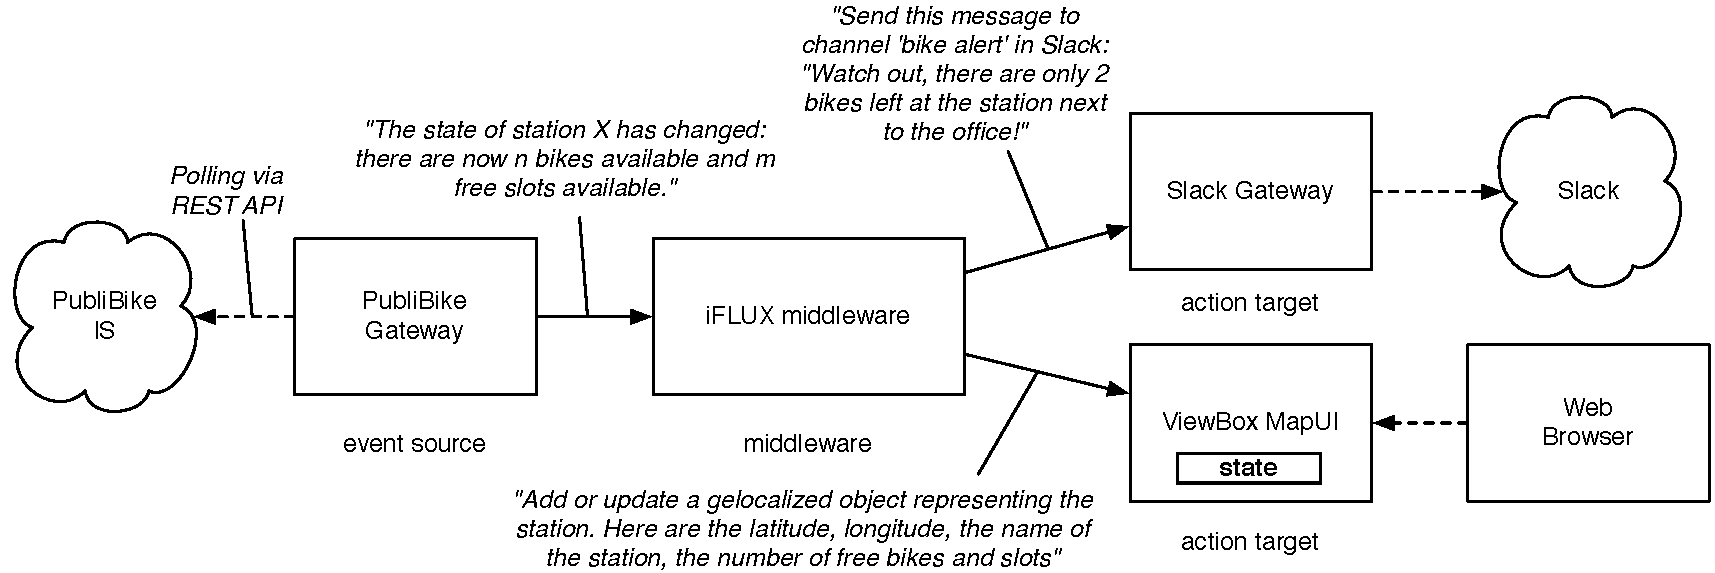
\includegraphics[width=0.7\textwidth]{figures/publibike.pdf}
\caption{The PubliBike application, with one event source and two action targets}
\label{fig:publibike}
\end{figure*}

\begin{figure*}
\centering
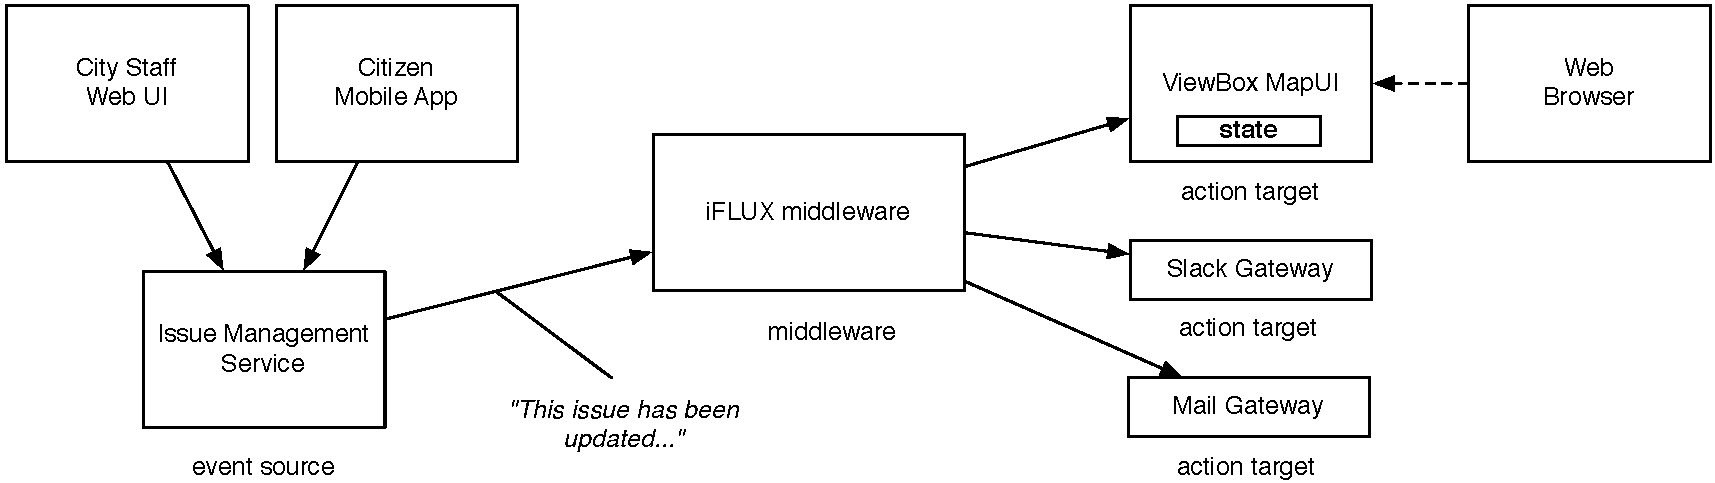
\includegraphics[width=0.7\textwidth]{figures/citizen}
\caption{The Citizen Engagement application, with one event source and three action targets}
\label{fig:citizen}
\end{figure*}

%\begin{figure*}
%\centering
%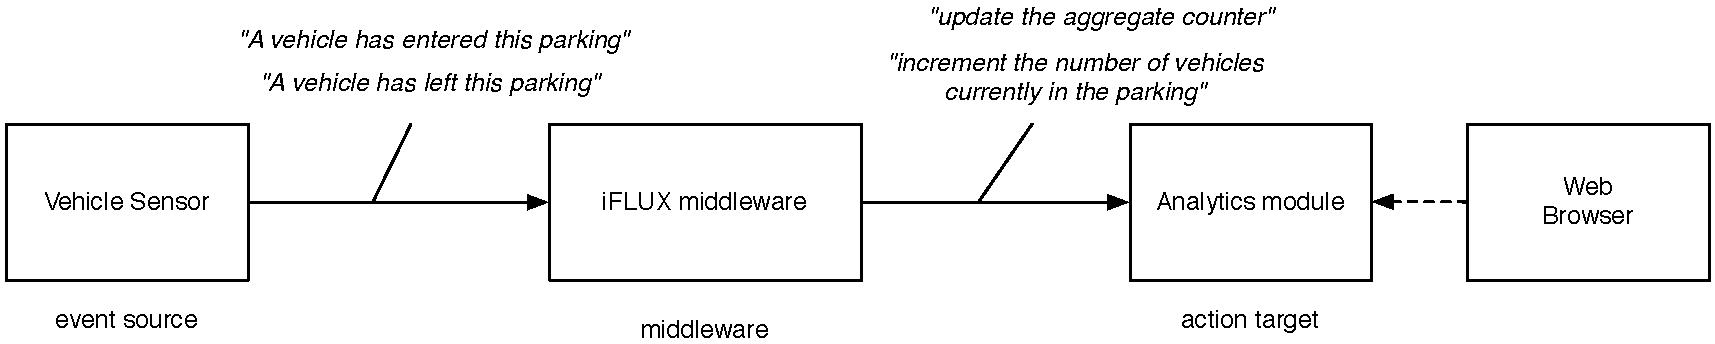
\includegraphics[width=0.9\textwidth]{figures/paleo}
%\caption{The Paléo Festival application, with one event source and one action target}
%\label{fig:paleo}
%\end{figure*}

%\begin{figure*}
%\centering
%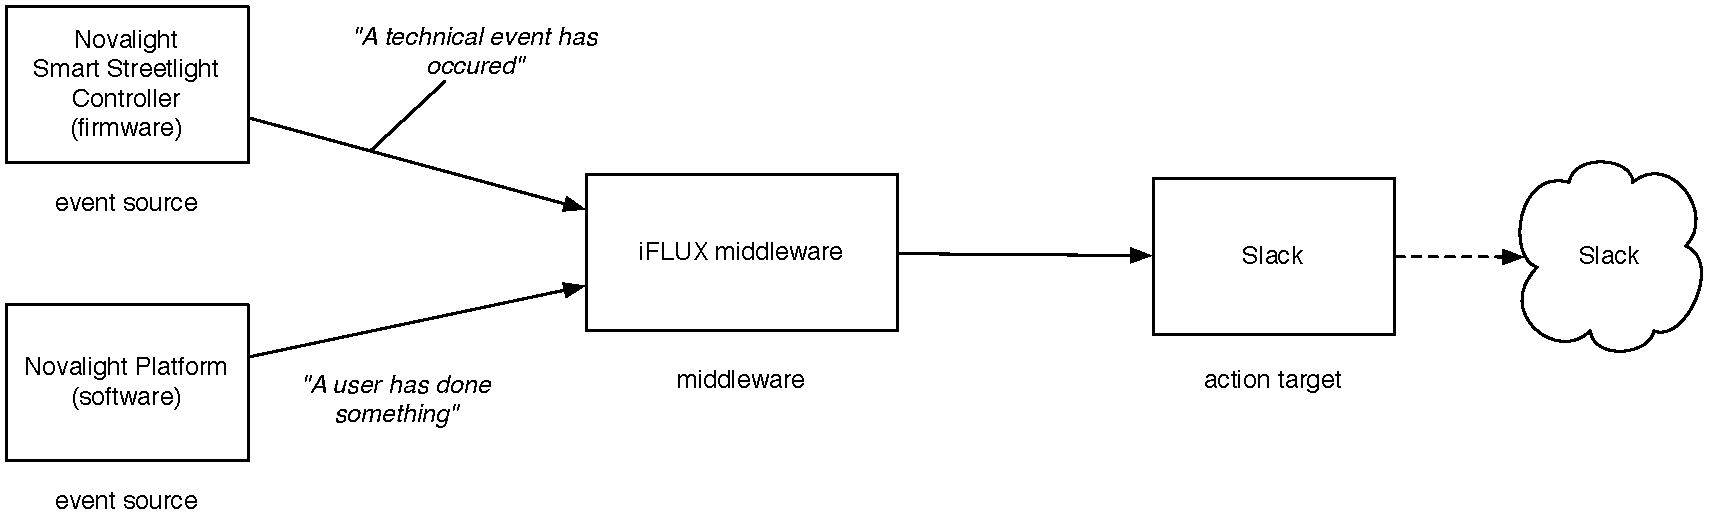
\includegraphics[width=0.9\textwidth]{figures/awareness}
%\caption{The Awareness @ Novaccess application, with two event sources and one action target}
%\label{fig:paleo}
%\end{figure*}


\subsection{PubliBike}

Like in many other countries, bike sharing stations are increasingly deployed in swiss cities (see Figure \ref{fig:publibikeStation}). Customers need to acquire a smart card, with which they can unlock a bike at a station. They also use the smart card when they later return the bike. The bike stations are connected to a nation-wide information system, named PubliBike. PubliBike makes it possible to know the number of available bikes and free slots at every station, in realtime. The data can be accessed via a REST API: the returned JSON payload contains the current state of all stations.

\begin{figure}[H]
\centering
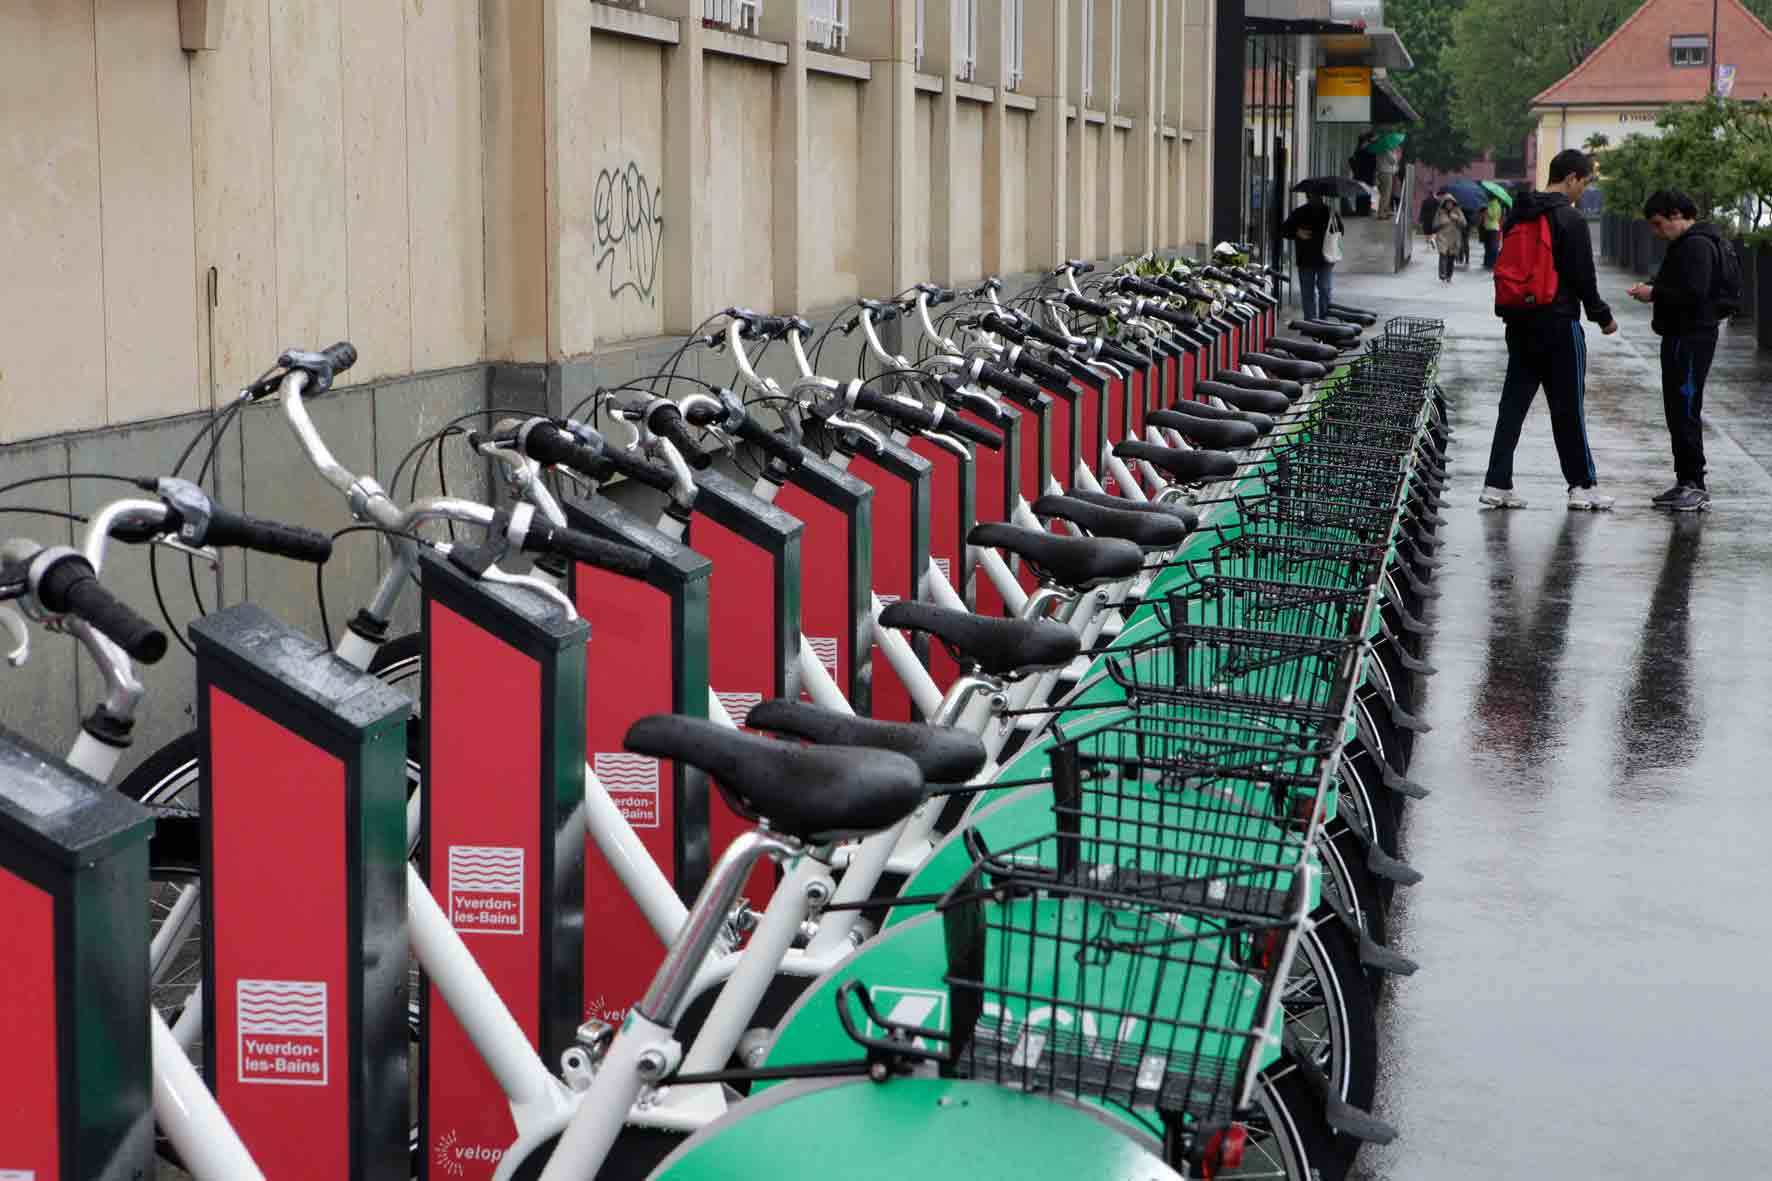
\includegraphics[width=0.85\columnwidth]{figures/publibikephoto2.jpg}
\caption{A bike station in Yverdon-les-Bains}
\label{fig:publibikeStation}
\end{figure}

\begin{figure}[H]
\centering
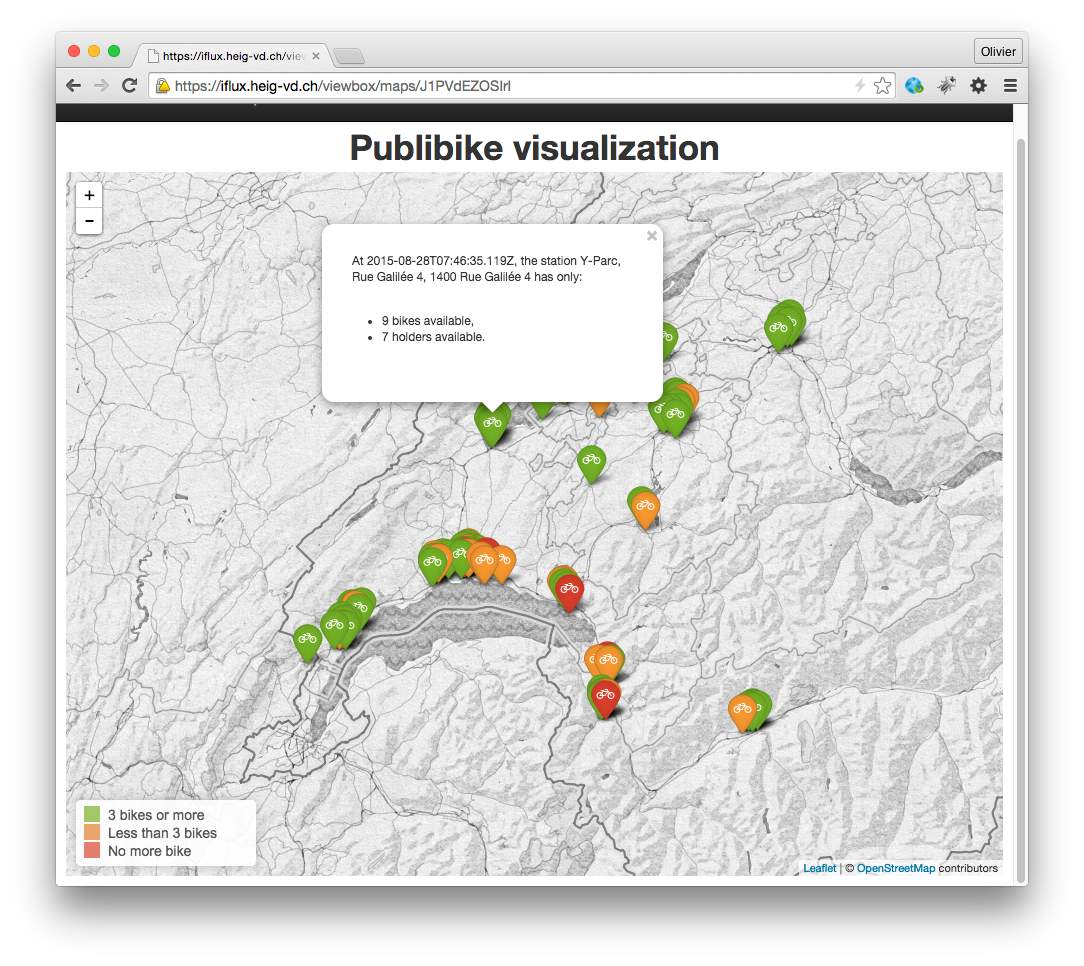
\includegraphics[width=0.75\columnwidth]{figures/publibike-viewbox.png}
\caption{Bike stations displayed by an action target}
\label{fig:publibikeMap}
\end{figure}


As illustrated in Figure \ref{fig:publibike}, we have implemented one \emph{event source} and two \emph{action targets} and we have defined rules in order to react to the activity monitored within the PubliBike system. These components are described in the following paragraphs.

\subsubsection{Tracking bike arrival and departure: the PubliBike Event Source}
Integrating PubliBike into the iFLUX ecosystem has first been achieved by defining a new \emph{event source} and by specifying the type of events produced by this source. Note that when doing this, we did not need to think about how the information would be used. It could be used to trigger alerts, to create visual representations, to compute statistics. As developers of the \emph{event source}, this is not something that we had to worry about (decoupling). We could have decided to define one \emph{event source} for every bike station, but instead we have preferred to define a single \emph{event source}: the PubliBike gateway, which is responsible for polling data via the PubliBike API and to detect state changes. In this scenario, while there are sensors and communication modules embedded in the physical stations, the iFLUX \emph{event source} is purely implemented in a software daemon running in the cloud. With the PubliBike \emph{event source} deployed, iFLUX receives an incoming stream of events, where every event represents a state change at a given station (i.e. either a bike has arrived or left). In addition to a timestamp, the events contain the following properties: the identifier, name and geographic coordinates of the station, the number of available bikes and the number of free slots. 

\subsubsection{Notifying users: the Slack action target}
Someone who uses the bike sharing service to commute from the office to the train station might be interested to be notified if the number of available bikes close to the office falls below a certain threshold. This person might also be interested to receive an alert if the number of free slots at the station falls below a threshold. To implement this use case, the user needs an iFLUX \emph{action target} that provides a bridge to a notification system (SMS, e-mail, etc.). To illustrate the idea, we have implemented an action target that makes it possible to send a notification in the Slack instant messaging platform \cite{slack}. The payloads sent to the action target via the REST API contain the message and the name of the channel where to post it. 

This allows the user to define an iFLUX rule, which states that \emph{\textbf{IF} an event is received from the PubliBike event source AND the event property `stationId' of the event is the one of the station close to my office AND if the event property `numberOfAvailableBike' is less than 3 \textbf{THEN} send an action to the Slack action target, with the property `channel' set to `bike alerts' and the property `message' set to `WARNING: there are not many bikes left at the station!'}. 

\subsubsection{Map visualization: the ViewBox action target}
Another idea for using the data produced by the PubliBike event source was to create a visual representation, where the current state of every bike station is shown on a geographical map (see Figure \ref{fig:publibikeMap}). This use case is interesting, because it raises the question about how to deal with application state given that iFLUX rules are stateless.

We have implemented an \emph{action target} that we have named the \emph{ViewBox action target}. Note that while it can be used in conjunction with the \emph{PubliBike event source}, it is generic and can be used with other types of \emph{event sources} (for instance, it has been used in the citizen engagement application described later). Essentially, the \emph{ViewBox action target} is responsible for managing application state, which is defined by a collection of geolocalized objects, which can have arbitrary properties attached to them. It accepts action payloads with the following properties: the unique identifier of a geolocalized object, the current latitude and longitude and a list of application specific values (in the case of PubliBike, the name of the station and the number of available bikes and slots). When it receives an action via the REST endpoint, it creates or updates a geolocalized object with the property values in the payload. The \emph{action target} provides its own API (outside the scope of iFLUX), so that web browsers can fetch annotated maps. 

After deploying the \emph{Viewbox action target}, we were able to configure a rule so that whenever an event was received from the \emph{PubliBike event source}, an action would be sent to the \emph{ViewBox action target} to update the corresponding geolocalized object.


%\FloatBarrier



\subsection{Citizen Engagement}

After a few months of work on iFLUX, we used the platform in a two-weeks undergraduate course dedicated to end-to-end mobile services. The course is project-oriented and every year, we use an application domain to provide some context to the students. This year, we explained that software platforms are increasingly deployed, so that citizen can report issues to city authorities \cite{patel2015guide,offenhuber2014infrastructure}. Users can report broken street lights, graffitis, dangerous areas, etc. The students were asked to design a system with two components. Firstly, they had to implement a simple issue tracking system and to expose their domain model via a RESTful API. Secondly, they had to implement a mobile app that would be provided to citizen, so that they could easily report issues and follow their resolution process.

The Citizen Engagement back-end was then transformed into an iFLUX \emph{event source}. This was done by emitting an event whenever the state of an issue would change (created, acknowledged, in progress, resolved, etc.). Special properties were added to the event (e.g. to attach comments to state transitions). Again, since emitting an iFLUX event is not more complicated than issuing a POST request, the integration was trivial. 
%As illustrated in Figure \ref{fig:citizenEngagement}, 
We were then able to combine the new \emph{event source} with existing \emph{action targets}. It was really easy to implement a workflow to notify city staff about new issues, either via Slack or via email. It was also very easy to create a map to visualize the issue with the \emph{Viewbox action target} described before. Figure \ref{fig:citizen} shows the end-to-end workflow in iFLUX. Several rules have been added to trigger behavior in the action targets whenever an issue is updated.

%\begin{figure}
%\centering
%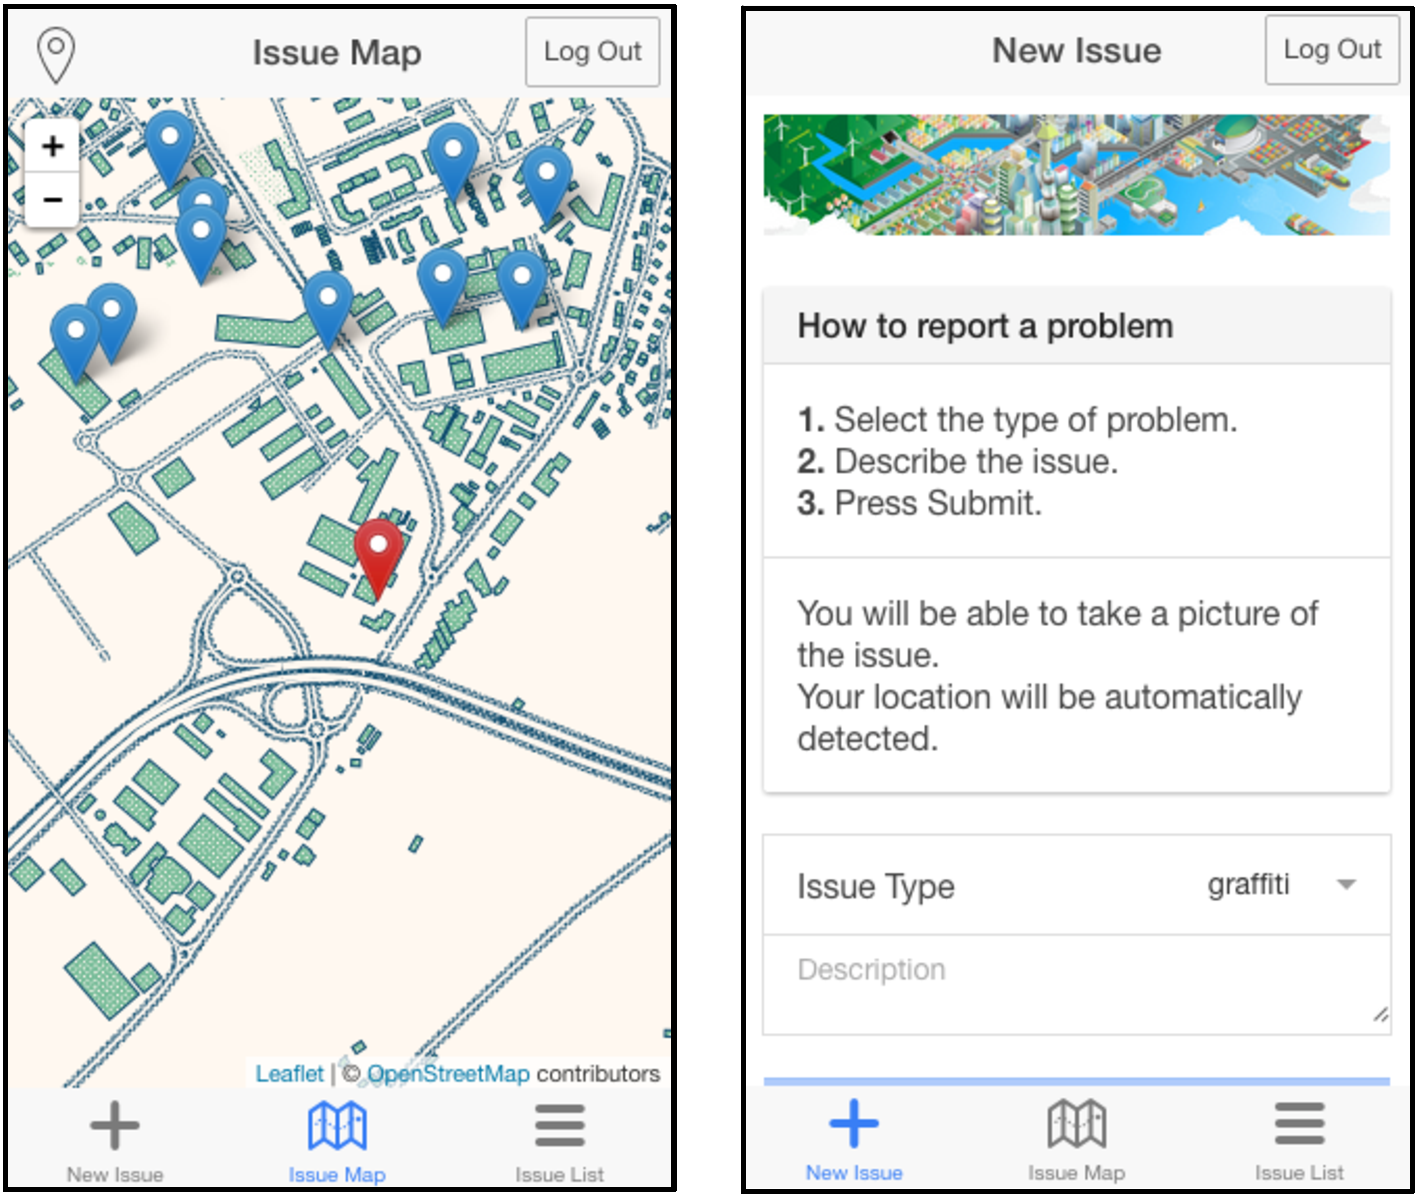
\includegraphics[width=0.8\columnwidth]{figures/citizen-mobile.pdf}
%\caption{The mobile app used to report issues}
%\label{fig:citizenMobile}
%\end{figure}


%\begin{figure}
%\centering
%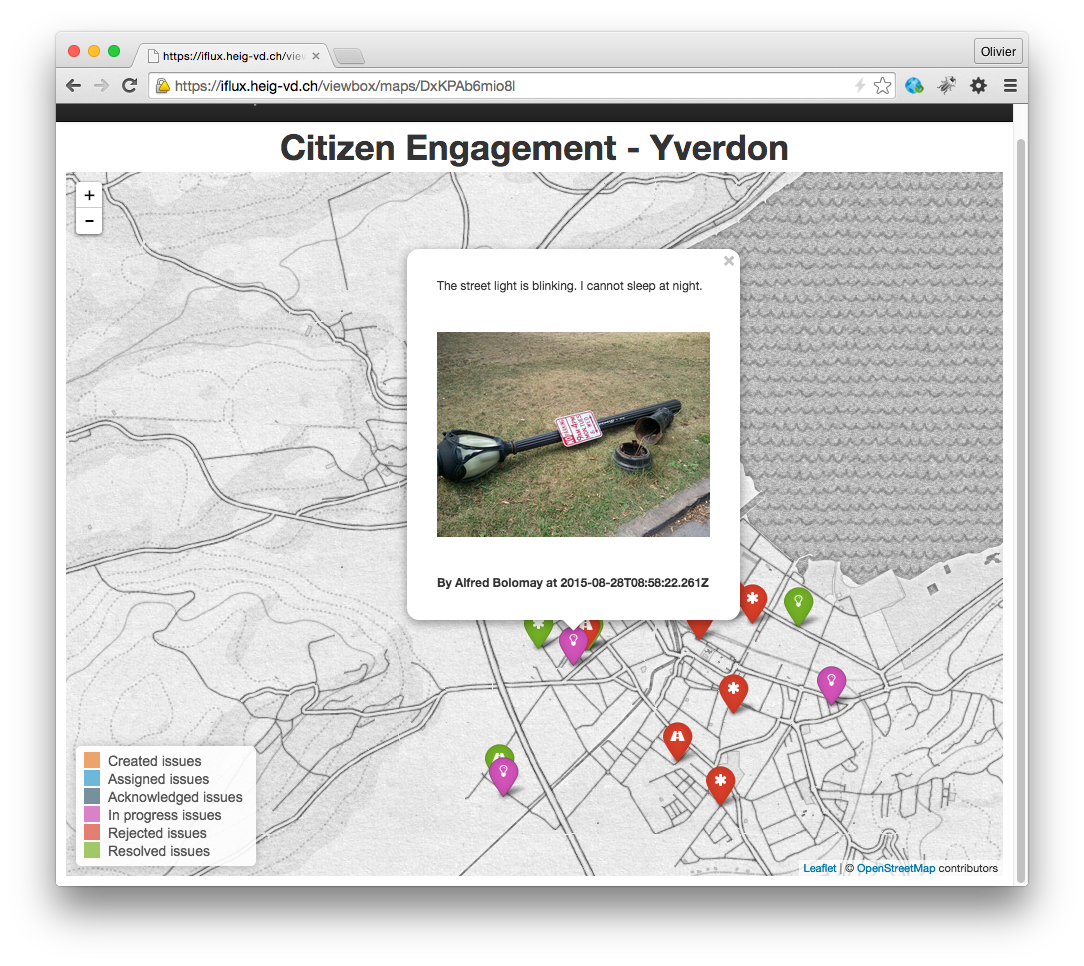
\includegraphics[width=0.9\columnwidth]{figures/citizen-viewbox.png}
%\caption{Issues shown by the ViewBox action target}
%\label{fig:citizenMap}
%\end{figure}

%\begin{figure}
%\centering
%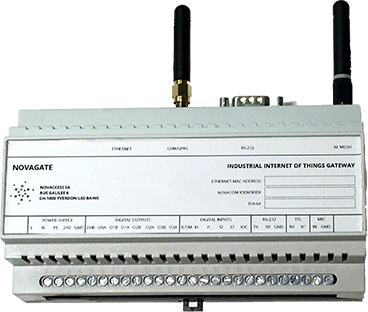
\includegraphics[width=0.8\columnwidth]{figures/novagate.png}
%\caption{The Novaccess IoT gateway is an iFLUX event source}
%\label{fig:novagate}
%\end{figure}


\subsection{Parking @ Paléo}

Paléo Festival is one of the largest music festivals in Switzerland. This year, had the opportunity to evaluate several iNUIT projects in a proof-of-concept deployment. One need expressed by the organizers was to get realtime information about the flow of vehicles and the occupancy of the parkings. To address this question, we created a system composed of one iFLUX \emph{event source} and one iFLUX \emph{action target}. 

The \emph{event source} is a smart object located at the entrance of the parking (see Figure \ref{fig:paleo}), which detects vehicles with ultrasonic sensors. Connected to the Internet via a 802.15.4 mesh network and a WoT gateway, the object emits an event every time a car enters or leaves the parking. The \emph{action target} is responsible for managing application state, which consists of the number of cars currently in the parking, as well as aggregate metrics about the flow of vehicles (number of entries and departures per minute, hour and day). The \emph{action target} publishes this information via a custom REST API, which is used by a web dashboard.

\begin{figure}
\centering
%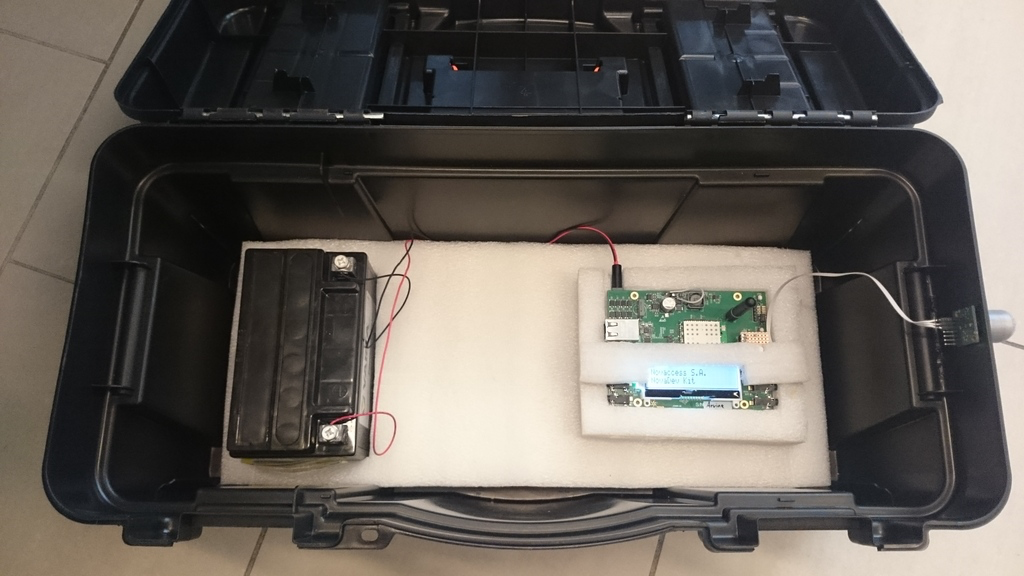
\includegraphics[width=0.9\columnwidth]{figures/paleo-before.png}
%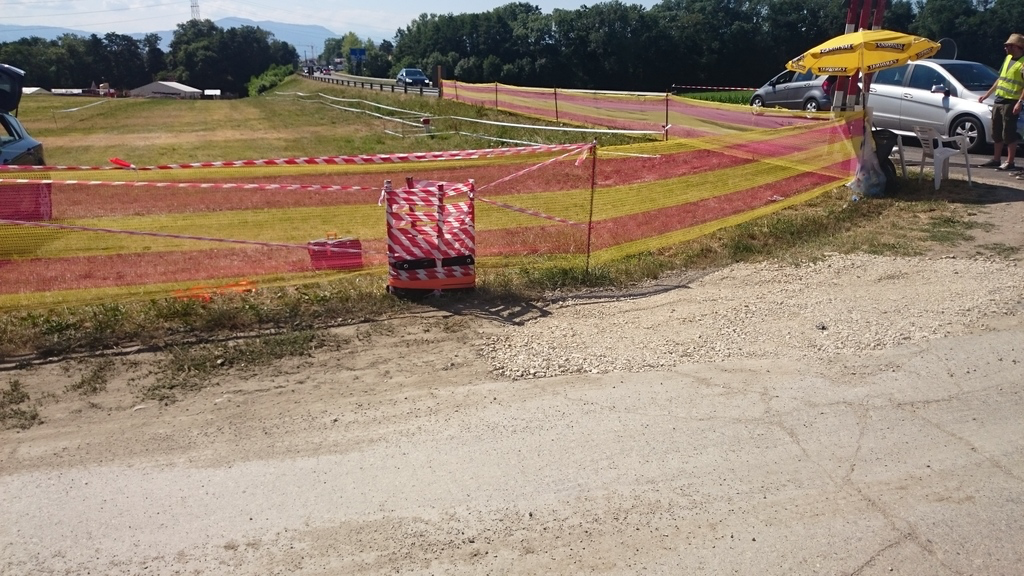
\includegraphics[width=0.9\columnwidth]{figures/paleo-during.png}
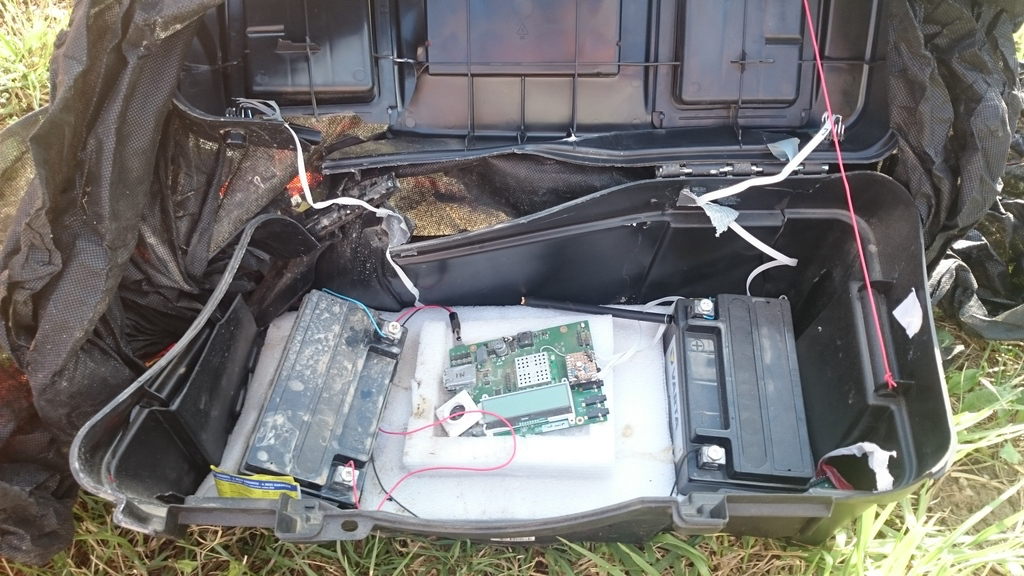
\includegraphics[width=0.85\columnwidth]{figures/paleo-after.png}
\caption{The event source after the festival}
\label{fig:paleo}
\end{figure}


\subsection{Awareness @ Novaccess}

Novaccess is a startup which develops an integrated stack (hardware, firmware, software) for the industrial Internet of Things. Novaccess has developed NovaLight, a smart lighting solution, which allows municipalities to reduce costs by lowering energy consumption and improving maintenance procedures. Measures are collected from street lights (consumption, faults, etc.) and analyzed. The platform can also dynamically and remotely adjust lighting levels.

%\emph{Awareness} is a concept that has been studied extensively in the Computer Supported Cooperative Work (CSCW) literature. While awareness is a somewhat broad concept, with several definitions, we like to think of it as a general sense of what is happening in a particular environment. In the context of Novalight, \emph{awareness} means that the Novaccess team would like to get a better sense about what is happening, on a continuous basis and without effort. The team would like to be able to detect unusual or interesting patterns. There are actually different dimensions that the team would like to be aware of. For example, Novaccess product owners would like to get a sense of the activity of end-users (are they using the web front-end, are they facing issues, are there features that they use a lot, etc.). Also, Novaccess engineers would like to get a sense of the technical activity (are there communication issues, are there faulty components to replace, what is the amount of transmitted commands, etc.).

We have worked with the Novaccess team to develop an \emph{awareness system} with iFLUX, i.e. a system which collects various types of events and generates notifications for the Novaccess staff. Several \emph{event sources} have been created. The first source, embedded in the NovaLight software, emits events that correspond to user actions (e.g. user has logged in, user has sent a command to a street light, etc.) or to technical issues (e.g. the database size has reached a given threshold). The second source, embedded in the NovaLight IoT gateway, emits events that correspond to measures or technical issues. The \emph{action target} used in the system is the Slack gateway presented before. Rules have been configured on the iFLUX middleware to send the text notifications via Slack, when \emph{interesting} events happen. The flexibility of the setup comes from the fact that it is possible to configure more than a rule. This allows the team to fine tune the amount and destination of the generated awareness messages. This simple setup could easily be extended with other notification devices (lava lamps, color LEDs, etc.).



\section{Conclusions}

We have introduced iFLUX, a middleware that enables a lightweight integration of loosely coupled services. Developed in the context of Smart Cities, it is applicable to other domains. iFLUX is particularly well suited to facilitate prototyping and co-design activities in WoT environments. Hopefully, the examples have shown that bringing an existing component (a smart object, a WoT gateway or a software application) into the iFLUX ecosystem is quick and easy. Even if iFLUX is currently based on stateless Event-Condition-Action rules, we have evidence that valuable workflows can already be implemented from the system. Still, we are currently extending the programming model to support stateful rules. This raises new types of issues, in terms of scalability and performance. Last but not least, iFLUX is an open source project. More information is available at \url{www.iflux.io}.



%\end{document}  % This is where a 'short' article might terminate

%ACKNOWLEDGMENTS are optional
%\section{Acknowledgments}
%Funding for the iFLUX project has been provided by the HES-SO University of Applied Sciences Western Switerland, as part of the iNUIT Smart City research program.

%
% The following two commands are all you need in the
% initial runs of your .tex file to
% produce the bibliography for the citations in your paper.
\bibliographystyle{abbrv}
\bibliography{bibliography}  % bibliography.bib is the name of the Bibliography in this case
% You must have a proper ".bib" file
%  and remember to run:
% latex bibtex latex latex
% to resolve all references
%
% ACM needs 'a single self-contained file'!
%


\end{document}
